\documentclass[a4paper,man, natbib,floatsintext]{apa6} %apa6/jou/man/doc

\usepackage[english]{babel}
\usepackage{csquotes}
\MakeOuterQuote{"} %will substitute " with quotes `` ''
\usepackage[utf8x]{inputenc}
\usepackage{amsmath,amssymb}
\usepackage{graphicx}
\usepackage[colorinlistoftodos]{todonotes}

\usepackage{multicol}
\usepackage{multirow}
\usepackage{booktabs}
\usepackage{tabularx}
\usepackage{setspace}% http://ctan.org/pkg/setspace
\usepackage{url}
%This makes urls break at the end of a line
\makeatletter
\g@addto@macro{\UrlBreaks}{\UrlOrds}
\makeatother
\usepackage{rotating}
\usepackage[toc,page]{appendix}
\addto{\captionsenglish}{\renewcommand*{\appendixname}{Supplement}}
\usepackage{color}
\usepackage{subscript}
\usepackage{threeparttable}
\usepackage{threeparttablex}
\usepackage{longtable}
\usepackage{dcolumn}
\usepackage{longtable}
\usepackage{times}
\usepackage{lipsum}
% \AtBeginEnvironment{tabular}{\singlespacing}% Single spacing in tabular environment
% \AtBeginEnvironment{caption}{\doublespacing}% Single spacing in tabular environment



\newcommand{\refs}{\textcolor{red}{(REF)}}

\title{Deconstructing financial risk perception: Risk as loss explains the risk-return paradox}
\shorttitle{Deconstructing financial risks}

\threeauthors{Jana B. Jarecki}{Janine Hoffart}{Jörg Rieskamp}
\affiliation{University of Basel}

% \leftheader{Deconstructing risk}

\abstract{
Incorrect beliefs of individuals about the risks of investments are disadvantageous in an increasingly complex financial world. A commonly-held incorrect belief is the perception that high-risk investments have low returns (risk-return paradox). This perception is contrary to financial markets, where the returns of assets increase with the risk, measured as outcome variance (risk premium). In two studies we examined the cognitive underpinnings of this bias in risk and return perception. Study 1 (\textit{N}=96) explains the bias as by-product of the semantics of risk. We hypothesized and found that people's understanding of the term risk to mean loss, not variance, explains the risk-return paradox. The paradox vanished, as soon as the beliefs about investment variance were conceptualized as fluctuation instead of risk. Results from quantitative statistical analysis and qualitative content analysis strongly suggest that a semantic analysis of risk perception explains the risk-return paradox. Study~2 (\textit{N}=242) replicates Study 1 and examines the moderators information and attitudes. The results show that providing information about investments is necessary in order to de-bias the risk-return paradox by conceptualizing risk as fluctuation. Regarding attitudes, we find that positive attitudes are associated with lower "risk" perceptions, as predicted by the affect heuristic. However "fluctuation" perceptions are unaffected by attitudes, when information about investments is given. If no information about investments is given, risk- and return judgments are less accurate and attitudes influence perceptions substantially. Our results highlight the role of semantics in apparent paradoxes of risk perception and suggest the usage of unambiguous terms (like fluctuation) to measure variance perceptions in the financial domain.}
\keywords{risk--return paradox; risk perception; attitudes; affect heuristic, risk--return belief, stock market}

\authornote{This research is supported by a grant (SNF \# 143854) of the Swiss National Science Foundation to the second and third author. \textcolor{red}{Please check if this info is correct. Also: should I (Jana) be corresponding author, rather?}

Correspondence concerning this article should be addressed to Janine Christin Hoffart. University of Basel, Department of Psychology, Missionsstrasse 62a, 4055 Basel, Switzerland.  E-mail: janine.hoffart@unibas.ch
}

\begin{document}
\urlstyle{same}
\maketitle%
%
Poor financial literacy is an important issue, which has been making headlines for 80 years \citep{carrns2019,nyt1939}. Many societies strive for an economy in which everybody makes "informed financial decisions" \citep[][p. 6]{FinancialLitear2011} and ample efforts worldwide have been made to increase financial literacy \citep{OECD2019}. One highly important aspect of well-informed financial choices concerns people's understanding of the risks in relation to the  benefits of financial investments. Risk comprehension is considered paramount to good economic choices. To facilitate the understanding of the risks of investments, major financial institutions have started to provide potential investors with simplified information about the risks of investments, such as risk categories from low risk to high risk \citep[e.g., ][]{postfinance2019}, in the hope to improve people's understanding of the true risks (outcome variances) associated with different investments.

Risk has a clear definition in economic theory and finance, namely the \textit{variance} (expected squared deviation from the mean), or semi-variance of the distribution of returns on investments, and this definition is widely used by psychologists and neuroscientists \citep[e.g.,][]{Nosic2010, Coombs1960, Mishra2016,Rushworth2008, Preuschoff2006, Fujimoto2016}. Any communication of "risk" in the sense of this economic notion of risk as variance comes with the underlying assumption that the majority of individual decision makers, too, understand financial risks in terms of outcome variance.

\subsection{The risk-return paradox} Despite the efforts towards increased financial literacy, people seem to be biased in their understanding of financial risks (variance) and returns, and particularly regarding how risks relate to  returns \citep{Shefrin1995,Ganzach2000,Kempf2014}. Across industries, the financial market often offers a risk premium, with high-variance (risky) investments offering higher returns compared to less risky investments, in the expectation. This positive variance-return relation is in line with economic asset pricing models \citep[][]{Markowitz1952}, and it holds by and large in international stock markets \citep[][]{Dimson2003}.\footnote{In some markets there is a debate about the premium (REF TODO: Jana add references to BROMAN's paradox here).} Contrary to the risk premium, the vast majority of people seems to believe in a risk punishment, judging high-risk investments as low-return investments \citep[][]{Shefrin1995, Shefrin2000, Shefrin2001, Kempf2014, Ganzach2000}. The perceived negative risk-return relation, contrary to the market's positive relation, is know as \textit{risk-return paradox}. The risk-return paradox is a pervasive phenomenon \citep{Kempf2014,Ganzach2000}. People's risk-return ratings were negatively correlated in a variety of life domains besides finance, including technology and medicine \citep[e.g.][]{Fischhoff1978, Alhakami1994,Sokolowska2015,Fleming2012}. In financial contexts, research has shown that even investors and economic students, who can be considered experts, exhibit the risk-return paradox and rate subjectively high-risk stocks as being low-return stocks \citep{Kempf2014}. Om one study \citep{Shefrin1995} financial analysts and executives rated the returns of ten stock market companies in doing so they evaluated the companies with low variances (risk) as those with high returns.
%But the calculations were per asset class rather than across assets. In the study it is not clear how risk was operationalized. In study 3 risk was operationalized as costs. Unsurprisingly a negative correlation was found for laypeople, not for experts. For stem cell treatment, the authors found a negative cost-benefit correlation for laypeople and experts.
The risk-return paradox is thus a seemingly stable cognitive bias in the perception of risks (variances) and returns in many areas of life.

One academic explanation for the risk-return paradox in behavioral economics and judgment and decision making involves cognitive mechanisms that cause people to judge options by standards other than the objective information. The most common explanation suggests that attitudes drive risk-return perceptions \citep[some work indicates an influence of representativeness on risk perceptions,][but most work focuses on attitudes]{Shefrin1995, Shefrin2001, Pachur2012b}. In this context, attitudes refer to a global evaluative attitude toward an investment or technology (rather than a strong visceral response), including cognitive evaluations \citep[a global "good and bad"; ][]{Ganzach2000, Sjoerberg2007,Sokolowska2015}. In previous work, attitudes were found to moderate the strength of the psychological risk-return paradox \citep{Ganzach2000, Kempf2014, Finucane2000, Slovic2004}. The core assumption of the attitude-driven explanation is that those investments that receive a generally positive cognitive evaluation are predicted to be evaluated as having a lower risk and higher return, compared to more negatively evaluated investments. This effect of global attitudes on the perception of risk and return became known as the \textit{affect heuristic}  \citep{Finucane2000,Slovic2004}. It implies that people's general attitude towards assets should lead to a holistic evaluation of the asset and to correlated risk and return perceptions. Specifically, positive attitudes should lead to high-return-low-risk perceptions, and negative attitudes should lead to high-risk-low-return perceptions \citep{Ganzach2000, Finucane2000}.

However, the traditional attitude-driven academic view on the risk-return paradox, has neglected an important line of  research on risk: Evidence from semantic studies of the meaning and usage of the term "risk" have established a reliable notion of \textit{risks as losses}. In nonacademic language risk means unwanted events and their causes \citep[American English corpus from 1992-2012,][]{Boholm2016}. Loss, danger, and loss probabilities surround the term risk in practice. Contrary to the academic notion of risk as variance,  psychologically, risk is not understood as variance but as loss \citep[e.g.][]{Libby1977, Sachse2012}. Even managers view risks as related to loss \citep{Mohr2010, Duxbury2004, Shapira1995}, with low correlations between the perceived risk and the objective variance of options \citep{Weber2005,Klos2005a}. This shows that psychologically the concept of risk is much less clear than in the academic models of financial risks. Therefore, the present research investigates if the notion of risk as loss (the loss-semantics of risk) can provide an alternative explanation of the risk-return paradox.
%Keller et al., 1986; E.U. Weber, 1988, 1999; Sarin & M. Weber, 1993; Brachinger & M. Weber, 1997; Jia et al., 1999; Baz et al., 1999

The core assumption of our semantic view on risk perception and the risk-return paradox, is that the notion of risk as loss causes the risk-return paradox (the negative subjective risk-return correlation). Importantly, the semantics of risk-as-losses imply the risk-return paradox: If people understand risk as loss, their judgments of risks should correlate negatively with their return judgments, because loss and return are antonyms and further because a loss and a gain are generally two mutually exclusive outcomes of choices under risk. If this were true, people's supposedly biased risk-return perception can be considered a correct response to their interpretation of the term risk as loss (rather than as variance).  Further, people's literal "risk" judgment should reflect the real loss and the variance simultaneously, and therefore lead to noisy perceptions of the objective (true) variances of risky options.

%Conceptual support for this hypothesis comes from results form a multinational OECD survey, finding that being asked about the risk-return relation an abstract level rather than being asked to judge risks and returns of individual assets, 81\% of respondents correctly reported that taking financial risks increases returns (OECD/INFE International Survey on Adult Financial Literacy Competencies, 2016). This means that in the abstract, people are well aware of the risk premium, but not when judging individual investments' risks. 

% Sokolowska and Sleboda's \citeyear{Sokolowska2015} study, which showed the risk-return paradox for energy production technology, defined

% -------------------------------------------------------------------------------------------------
% Maybe necessary for later
%
% Another explanation is that participants rely on their subjective risk estimates, as it is implied by the risk-return framework. The \textit{risk--return framework} \citep{Weber1997} (risk-value framework) is a widespread psychological theory of decisions under risk \citep[e.g.,][]{Weber1999, Weber2008, Mohr2010, Sunden1998, Sarin1999, Hosker-Field2016, Jia1996}. It posits that risk taking is governed by perceived, rather than objective, levels of risks and perceived benefits, and a subjective trade off between high benefits and high risks. Predictions of the theory, such as that high risk judgment is associated with a lower willingness to engage in the risk, were supported  \citep{Blais2006, Blais2009, Wilke2014}. 
% Weber, Blais, and Betz \cite{Weber2002} 'we are interested in your gut level assessment of how risky each situation is. For each of the following statements, please indicate how risky you perceive each situation.' Participants may now either understand this as costs or as variance.
% Wilke: For each of the following statements, please indicate how risky you perceive each situation to be. Provide a rating from not risky at all to extremely risky, using the following scale: The fact that the perception of risks, rather than the objective variance, is a building block in the \textit{risk--return framework} \citep{Weber1997} renders it relevant for the current study. It is noteworthy, however, that the studies on the psychological risk--return framework asked participants for their perceived risk without defining it as either costs or variance. The research on the risk--return framework thus leaves it open if risks are merely perceived as costs, as indicated by the everyday language, or as variance.

%Crucially, in most studies on risk--return assumptions or the risk--return framework, participants were asked to judge how risky they perceive an option \citep[e.g.,][]{Kempf2014, Blais2006}. The 'objective' risk, against which people's responses were benchmarked, typically is variance. However, given that people often define risk as loss \citep{Duxbury2004, Sachse2012, Klos2005a}, people possibly did not understand the question precisely. Crucially, for effective communication between financial advisors and clients, it is important that both partners --advisors and clients-- have a common understanding of the concept of risk. Therefore, for Study one, we defined the goal to find a question that clearly measured variance. To do so, we assessed people's perception of return curves with various measures and identified which measure most accurately measures risk--as--variance. In Study 2, we replicated our findings from study one. In a separate condition, we increased uncertainty, by only showing people 
% -------------------------------------------------------------------------------------------------

In two studies we examined if the loss semantics of risks underlies risk-return paradox. Our experimental design contrasted different elicitation methods for the variance of investments (objective risk). Study~1 tested if the risk-return paradox is a by-product of the loss-semantics of the term risk. Study~2 extends the findings by investigating the influence of attitudes and fundamental information on risk.  Our work advances the literature on the risk-return paradox in three ways. We are, to the best of our knowledge, the first to show that measuring perceptions of variance without the influence of loss-semantics de-biases the risk-return paradox. Our work is ecologically valid, since our material consists of real stock and fund data \citep[as also][]{Kempf2014}.  Additionally, because methodologically the risk-return paradox is complicated by six-way inter-correlations\footnote{Real risk correlates with real return, perceived risk correlates with real risk,  perceived return correlates with real return, perceived risk correlates with real return, perceived return correlates with real risk}, we are the first to use partial correlation network analyses, which are specifically designed to analyze data with multi-way inter-correlations.

\subsection{Hypothesis}
The semantic view on risk perception holds that "risk" judgments are less accurate in terms of their correlation with the objective variances of risky options, compared to the accuracy of other measures of variance, which are less semantically related to loss (such as predictability, fluctuation, or variability). Therefore we predict that judgments of risk will be less accurate measurements of the objective variances of risky options than other measures of variance ($H_1$). Secondly, we hypothesize that the risk--return paradox (the negative correlation between perceived risk and perceived return), is based on the semantic confusion of risk with loss and therefore the paradox should occur mainly when people judge perceived "risk", but not when judging other measures of variance, which are less semantically related to loss (such as predictability, fluctuation, or variability) ($H_2$). No hypothesis were made about which of the alternative terms (predictability, fluctuation, or variability) would lead to the most precise perception of the objective order of magnitude of the variances of the stocks.

\section{Study 1}
Study~1 investigates if the loss semantics of the term risk causes the risk-return paradox. Aiming to disentangle the notion of loss from the perception of variance, the design of the present study manipulated the terms used to elicit the evaluations of the variance of stocks. Participants were asked about the perceived "risk" of a st of stocks as baseline measure; further they were asked about the "fluctuation", "variability (variance)", and "predictability" of those stocks, Predictability judgments have been shown to relate to financial risk perception \citep{Sachse2012}; and the other terms represent an intuitive notion of variance, which we hoped would be associated less with loss than the term "risk". Our study also assessed the perceptions of the losses and the returns of stocks.

\section{Methods}
\subsection{Participants}
In total 103 adult participants recruited from ClickWorker completed an online study, seven were excluded (for reporting inattentiveness or the task being unclear, or using only one response option throughout a scale), leaving a final sample of $N$ = 96; 56 males and 40 females (58\% and 42\%, respectively), mean age 37 years (Med = 34, $SD$ = 12, range 18-65 years). The dominant native language was $n =$ 90 German and $n=6$ other (94\% and 6\%, respectively), mean study completion time was 42 min (range $10$ to $120$ min), remuneration was 4.5 Euro (4.83 U.S. dollar at the time of the study). Data were collected in May 2017, the study was approved by the institutional review board at the University of Basel. All participants possessed a school degree, $n$ = 37 had a Bachelor’s or a higher degree; most participants were working full or part time, $n=10$ were students.

\subsection{Task Design}
The design was a 1 x 4 (question wording [risk, fluctuation, predictability, variability (variance)]) within-subject design. Participant rated 19 stocks that were presented graphically one by one, see Materials. Participants rated the perceived risk, perceived predictability, perceived  fluctuation, and perceived variability (variance) of all stocks. Participants also evaluated the stocks' expected loss, loss magnitude, loss probability, and return. Table \ref{table:Questions} shows the questions.

% Wie hoch schätzen Sie das Risiko der gezeigten Aktie ein? Wie hoch schätzen Sie die Variabilität (Varianz) der gezeigten Aktie ein? Wie hoch schätzen Sie die durchschnittliche Schwankung der Rendite der gezeigten Aktie ein? Wie hoch schätzen Sie die Vorhersagbarkeit der Rendite der gezeigte Aktie ein (gemessen ab 2003)?

\begin{table}[hb!]
\centering
\onehalfspacing
\begin{threeparttable}
\caption{Conditions (within-subject) and Question Wording in Study 1}
\small
\label{table:Questions}
\begin{tabularx}{\columnwidth}{p{1.7cm}p{2.9cm}p{7cm}r{0.5cm}}
Category & Condition & Question asked & Response format \\
\toprule
\multirow{7}{*}{Variance} & Risk & As how high do you estimate the risk of the displayed stock? & 7--point Likert \\
& Variability & As how high do you estimate the variability (variance) of the displayed stock? & 7--point Likert \\
&  Fluctuation & As how high do you estimate the average fluctuation of the displayed stock returns? & 7--point Likert \\ 
 & Predictability & As how high do you estimate the predictability of the displayed stock (starting from 2003)? & 7--point Likert \\
 \cmidrule{2-4}
\multirow{7}{*}{Loss} & Expected loss & As how high do you estimate the expected average loss of this stock? &  $\%$ points \\
     & Loss magnitude & As how high do you estimate the average loss of this stock? & $\%$ points\\
     & Loss probability & As how high do you estimate the probability of making a loss with this stock in a randomly selected year?\\
 \cmidrule{2-4}
\multirow{1}{*}{Return} & Return magnitude & As how high do you estimate the average return of this stock? & 7--point Likert \\
\bottomrule
\\
\end{tabularx}
\begin{tablenotes}
\small
\item
 \textit{Note}. The original question wording was in German (see Supplement~\ref{sup:study1_material}), Likert-type scales were unipolar from \textit{1 = low} through \textit{4 = moderate} to \textit{7 = high}, except the return scale, which was biploar from \textit{1=extremely large losses} to \textit{7=extremely large gains}.

\end{tablenotes}
\end{threeparttable}
\end{table}

\subsection{Procedure} The experiment was a computerized online study. Participants were familiarized with 19 stocks, each of which was presented as graphically (Figure~\ref{fig:study1_material}). The stock graphs were unlabeled to avoid familiarity effects. Participants evaluated each stock individually (for example, evaluating "risk"). A Likert-type scale (from \textit{1 = low} through \textit{4 = moderate} to \textit{7 = high}) measured the evaluations. After the evaluation of all stocks, participants evaluated the stocks with respect to a different term (for instance, "risk" in block 1, "fluctuation" in block 2, etc.). The order of the terms and stocks were randomized across participants. Participants were instructed to make relative judgments among the set of stocks to avoid usage of external reference anchors. Participants also evaluated the stocks' return and loss (numeric inputs from \textit{0 - 100}). Further, the participants defined risk (\textit{What does it mean to you if a stock has 'high risk'?}), reported their stock market experience and knowledge, took a graph literacy test \citep{Garcia-Retamero2013a}, and reported demographics. Data quality checks followed (comprehension of instructions, self-reported quality). Participants had to pass an attention check question before each block to ensure they knew what to evaluate next. Participants saw only the return history of the stocks but no names of the stocks, to avoid that familiarity biases risk-return judgments \citep{Ganzach2000}.

\subsection{Stimuli}
The stimulus material was based on real stock market data to ensure ecological validity. Study~1 used the daily values of the 19 most-traded  stocks in Switzerland (as of October 2016, between January 2003 and December 2015, see Supplement~\ref{sup:study1_material}). To characterize the stocks, we computed the stocks' objective annual returns, variance in returns, and their losses. Our  measure of return was the stock's change in value after a one-year holding period, for each day of a calendar year, averaged within calendar years.\footnote{Each stock's daily return of investment was calculated as the percentage earnings between end and start values after a year, for example for 2006: $ROI_{2006} = \frac{v_{2007}^{\text{close}} - v_{2006}^{\text{open}}}{v_{2006}^{\text{open}}}$, where $v_y$ is the stock value in year $y$ the start and end of the trading day ($v^{\text{open}}$, $v^{\text{close}}$, respectively), correcting for bank holidays. If it was a bank holiday the next trading day was used.}
Information about the stimuli (in terms of the computed annual returns on investment) were provided to participants in form of a graphical display (year by return in percent, Figure~\ref{fig:study1_material}) to be evaluated by participants. Participants were informed about the meaning of the return that the graphic displayed in the instructions (see Supplement~\ref{sup:study1_material}). Participants were not informed about the names of the stocks.

\begin{figure}[h!] \centering
    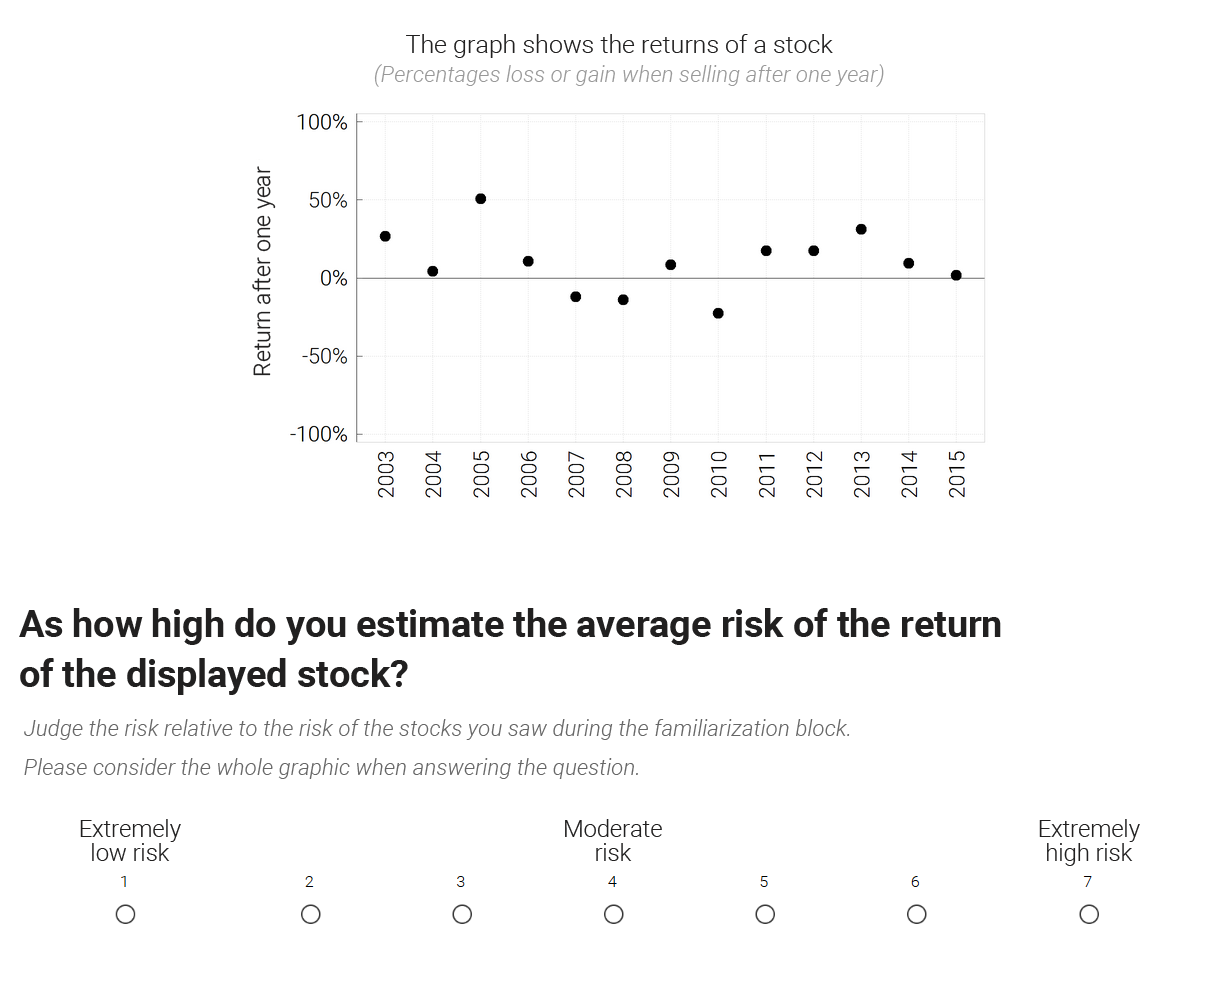
\includegraphics[width=0.85\textwidth]{fig1}
    \caption{\textit{Illustration of the Task in Study~1 and Study~2.} The original language of the study was German  (original wording: Supplement~\ref{sup:study1_material}), the English translation was added for this publication only. During Study~1, each participant evaluated 19 stocks with respect to variance-related terms in Table~\ref{table:Questions}: variability, risk, fluctuation, and predictability.}
    \label{fig:study1_material}
\end{figure}

\subsection{Analytical Approach}
Condition-related differences in the accuracy of the evaluation of the true variance---i.e., if perceived "risk" measures objective variances better than the other terms---was analyzed by a comparison among separate linear mixed-effects regression models, which included the predictors question condition, evaluation, the condition x evaluation interaction, and a by-participant random intercept and random slope to account for the clustering in the data \citep[following][]{Judd2017}.\footnote{The design of Study~1 has fully-crossed explanatory variables: each participant evaluated each stock in each condition once.} To investigate the effect of the question wording on the risk-return paradox, we employed two analysis. First, we report mixed-effects linear regression analyses The results of our regression analysis \citep[following][]{Judd2017,Barr2013a}, using the maximal model that converged. We predicted the perceived return from the predictors perceived-variance (z-standardized) $+$ condition (effect-coded) $+$ perceived-variance$\times$condition $+$ stock-return $+$ stock-return$\times$condition, including random effects (by-participant intercept $+$ by-participant slope for perceived-variance$\times$condition; uncorrelated random intercept and slope). The condition was effect-coded, effect-coding means that the coefficients represent the deviation from the grand mean rather than from a reference level. Technically, effect coding involves coding categorical variables such that the coefficients sum to zero, which facilitates the interpretation of interactions \citep[e.g.,][]{SingmannForthcoming}. In a second analysis we modeled the data by partial correlation networks \citep[e.g.,][]{Epskamp2019}, which provide insights into the conditional dependencies between multiple variables (i.e., the dependencies among perceived risk, objective risk, perceived return and objective return), we used hierarchical networks which also account for the the hierarchical structure of the data (within-subject design). We employed a random-intercept model.\footnote{The latest hierarchical network model, version 0.4.3, only allows random intercepts.} We further ran robustness checks, using sub-group analysis by means of partial correlation networks to control for the influence of graph literacy and expertise. Lastly, to gauge the relationship between participants' explicit definitions of "risk" and the strength of their risk-return paradox, we combined qualitative content analysis results with the partial correlation network analysis.

All analyses were conducted in R (v3.6.1 \citep{R}, using the packages lme4 v1.1 \citep{Bates2015}, and mlVAR v0.4.3 \citep{Epskamp2019}). Likert-type scale responses were z-standardized by participant to control for differences in scale use, except where stated otherwise, for a lack of convergence of models.


\subsection{Results}
% Our main analysis will test if we find the risk-return paradox in our data and how the paradox relates to the evaluation of "risk" in comparison to other terms. The first analysis tests which of the different terms leads to evaluations that correspond best to the objective variance of the stocks that people evaluated. 

\subsubsection{Accuracy of the perceived risk measures}
How well do the different evaluations (risk, fluctuation, variability (variance), and  predictability) represent the order of magnitude of the (objective) variances across the stocks? $H_1$ expects the perceptions of risk to be the least accurate measure of the objective variances compared to the perceptions of predictability, fluctuation, or variability. The (absolute) Pearson correlations between the stocks' objective variance and people's perceptions are ranked as: fluctuation $>$ variability $>$ predictability $>$ risk ($r_{fluct}=.69$, $r_{vari}=.64$, $r_{pred}= -.52$, $r_{risk}= .49$, respectively), pooled across participants and stocks (statistical tests can be found in Supplement~\ref{study1_risk-variance-correlation}). The regression model comparison 
%of the objective variances as a function of question wording condition and perception using a linear mixed-effects model \citep[following][]{Judd2017}\footnote{
%Dependent variable: the stock's objective variance in returns. Predictors: question, perception, and their interaction.
%Note, the objective variance is measured by index, but the predictors are measured by condition, index, and participant. This means predicting a group-level outcome from individual-level data, for which a linear mixed-effects model is not suitable, but structural equation modeling \citep{Croon2007}.
%},
% which accounts for clustering within participants, confirms the simple correlation result
(Table \ref{tab:study1_lm_results}) reveals that, as hypothesized, the model that includes perceived risk as predictor of objective variances has the worst fit, the best-fitting model uses perceived fluctuation as predictor of objective variance, as indicated by log likelihood, AIC, and BIC, and evidence strength \citep[the best model has an AIC weight of 1, see][]{Wagenmakers2004}. The regression coefficients show that all perceived values were positively related to the objective variance of the shown stocks. The highest standardized $\beta$ coefficient was obtained for perceived fluctuation ($\beta = 0.64$, one standard deviation change in the objective variance given one standard deviation change in the predictor, not shown in the table), the $\beta$s of variability, predictability, and risk were lower, $ 0.57, -0.39$, and $0.29$ (respectively). These results confirm $H_1$ according to whieh risk perceptions will reflect objective variances least accurately, and are in line with \citeauthor{Klos2005a}'s (\citeyear{Klos2005a}).


% Table created by stargazer v.5.2.2 by Marek Hlavac, Harvard University. E-mail: hlavac at fas.harvard.edu
% Date and time: Fr., Mai 17, 2019 - 10:13:52
\begin{table}[!htbp] \centering 
  \caption{Hierarchical linear model results, dependent variable: objective variance of shown stocks} 
  \label{tab:study1_lm_results} 
\begin{tabular}{@{\extracolsep{5pt}}lcccc} 
\\[-1.8ex]\hline 
\hline \\[-1.8ex] 
 & \multicolumn{4}{c}{Unstandardized b coefficients [range of dep. var. 0.014 $-$ 0.275]} \\ 
\cline{2-5} 
\\[-1.8ex] & (1) & (2) & (3) & (4)\\ 
\hline \\[-1.8ex] 
 Fluctuation & .028 &  &  &  \\ 
  & (.027, .030) &  &  &  \\ 
  & t = 32.413$^{***}$ &  &  &  \\ 
  & & & & \\ 
 Variability &  & .026 &  &  \\ 
  &  & (.024, .028) &  &  \\ 
  &  & t = 28.657$^{***}$ &  &  \\ 
  & & & & \\ 
 Predictability &  &  & $-$.017 &  \\ 
  &  &  & ($-$.019, $-$.015) &  \\ 
  &  &  & t = $-$17.359$^{***}$ &  \\ 
  & & & & \\ 
 Risk &  &  &  & .021 \\ 
  &  &  &  & (.018, .023) \\ 
  &  &  &  & t = 15.006$^{***}$ \\ 
  & & & & \\ 
 Constant & $-$.040 & $-$.026 & .158 & .009 \\ 
  & ($-$.048, $-$.031) & ($-$.034, $-$.017) & (.150, .165) & ($-$.003, .021) \\ 
  & t = $-$9.148$^{***}$ & t = $-$6.068$^{***}$ & t = 40.864$^{***}$ & t = 1.522 \\ 
  & & & & \\ 
\hline \\[-1.8ex] 
AIC weight$^{+}$ & 1.00 & 0.00 & 0.00 & 0.00 \\ 
AIC & -5458 & -5373 & -5027 & -4887 \\ 
BIC & -5425 & -5340 & -4994 & -4854 \\ 
LogLik & 2735 & 2692 & 2519 & 2449 \\ 
\hline 
\hline \\[-1.8ex] 
\textit{Note:}  & \multicolumn{4}{l}{$^{*}$p$<$0.05; $^{**}$p$<$0.01; $^{***}$p$<$0.001} \\ 
 & \multicolumn{4}{l}{$^{+}$Relative evidence strength, range 0-1 {\citep{Wagenmakers2004}}} \\ 
 & \multicolumn{4}{l}{Predictors are z-transformed} \\ 
 & \multicolumn{4}{l}{Model: random intercept and slope by subject; fit: restricted maximum likelihood.} \\ 
\end{tabular} 
\end{table} 


% \begin{table}[tbp]
% \begin{center}
% \begin{threeparttable}
% \begin{tabular}{lllll}
% \toprule
% contrast & \multicolumn{1}{c}{estimate} & \multicolumn{1}{c}{SE} & \multicolumn{1}{c}{z.ratio} & \multicolumn{1}{c}{p.value}\\
% \midrule
% Fluctuation - Risk & 0.002 & 0.001 & 1.336 & 0.540\\
% Fluctuation - Variability & 0.001 & 0.001 & 1.060 & 0.714\\
% Fluctuation - Predictability & 0.047 & 0.002 & 21.455 & 0.000\\
% Risk - Variability & 0.000 & 0.001 & -0.241 & 0.995\\
% Risk - Predictability & 0.045 & 0.003 & 17.831 & 0.000\\
% Variability - Predictability & 0.046 & 0.002 & 21.219 & 0.000\\
% \bottomrule
% \end{tabular}
% \end{threeparttable}
% \end{center}
% \end{table}






\subsubsection{De-biasing the risk-return paradox}
Regarding the effect of the condition on the risk-return paradox, we expect the risk-return paradox in the risk condition, but not in the other conditions. The true returns of the stocks used in Study~1 showed a risk premium (as theoretically expected); objective $r_{\text{risk,return}} = .51$, 95\% CI $[.07$, $.78]$, $p = .027$, pooled across stocks, risk measured as variance in returns (Figure~\ref{fig:rrc}a). Figure~\ref{fig:rrc}b shows the perceived returns in relation to the perceived risk, variance, fluctuation, and predictability. As hypothesized and unlike the objectively positive risk-return correlation, perceived "risk" correlated negatively with perceived returns ($r = -.14$), exhibiting the risk-return paradox. However, perceived fluctuation and perceived variability correlated positively with perceived returns ($r = .10$, $r = .11$, resp.), and thus reflect the direction of the market correlation instead of showing a risk-return paradox (inferential statistics of the simple correlations are given in Supplement~\ref{study1_supplementary_results}, Table~\ref{sup:tab:study1_rrc}).
%
\begin{figure}[!htbp] 
 \centering
 \fitfigure[]{fig2.png} 
  \caption{\textit{Objective risk-return relationship compared to perceived "risk"-return relationship across four measures of perceived variance}. (a) Objective risk-return relation: returns increase with variances across the stocks. (b) Perceived relations between the perceived returns of stocks and four measures of perceived variance ("perceived values"): perceived \textit{risk}, perceived \textit{variability}, perceived \textit{fluctuation}, and perceived \textit{predictability} (measured on 7-point Likert-type scales, z-standardized at the individual level). Lines depict best-fitting linear regressions, pooled across participants.}
  \label{fig:rrc}
\end{figure}

The results of our regression analysis from the maximal model that converged\footnote{Note on the model specification: The maximal mixed-effects model, which some recommend to use \citep{Barr2013a}, has a more complex random effects structure \citep[see][]{Judd2017}. Specifying this full model caused singularity, i.e. degenerate parameter estimates, which is a convergence issue common to mixed-effects model involving by-participant \textit{and} by-stimulus random effects \citep{Bates2015b}. Singularity issues can severely distort the interpretation of the parameters \citep{Bates2015b}. Thus we simplified our model by following recommendations for mixed-effects modeling when the interaction is of interest \citep{Barr2013a}. Moreover, the full model also includes correlated random intercepts and slopes. A model with those also failed to converge, but simulations showed low Type-1 error rates for uncorrelated random effects \citep{Matuschek2017}.}
 %The results show that the perception changes with the question-wording condition (perception-condition itneraction effect, SSE$=26.898$, MSE$=8.966$, $F(3,185.773)=8.639$, $p$<$.001$) and also a main effect of perception (SSE$=16.201$, MSE$=16.201$, $F(1,94.998)=15.610$, $p$<$.001$).
reveal that, as hypothesized, only in the "risk" condition the perceived returns decrease with the perceived risks ($b_{risk}=-0.159$). No such paradox surfaced in the fluctuation or variability condition, $b_{fluct}=0.086$ and $b_{vari}=0.086$ (all $p$s$<.05$, Table~\ref{study1:mixed_effects_model}).
%The estimated marginal effects of the condition on the return perceptions are shown in Table~\ref{study1_lme_trends}. 
The perceptions of predictability were not significantly related to the perceptions of return. Similarly, the results from the partial correlation networks---which account for the six-way inter-correlations between the perceived and objective variables---show the risk-return paradox exclusively for perceived "risk", and for none of the other terms. Perceived risk decreased with perceived return ($r_{part} = -.15$, $p < .001$; Figure~\ref{fig:pcn}a). These results corroborate the results from the linear regression analyses.
 

\begin{table}[H]
\begin{center}
\begin{threeparttable}
\caption{Regression (mixed-effects model) with dependent variable: perceived return \\\label{study1:mixed_effects_model}}
    \begin{tabular}{lrcrcrr}
    \toprule
     & $b$ & 95\%\textit{CI} & $b^*$ & \textit{df} & \textit{t} & \textit{p}\\
    \midrule
    Constant & 4.604 & [4.456,4.763] & --- & 95.005 & 60.936 & $<$ .001\\
    Perception & 0.009 & [-0.032,0.051] & 0.007 & 375.787 & 0.455 & .650\\
    Perception x Risk & -0.159 & [0.013,0.156] & -0.084 & 178.275 & -4.716 & $<$ .001\\
    Perception x Fluctuation & 0.086 & [-0.226,-0.097] & 0.046 & 164.840 & 2.445 & .016\\
    Perception x Variability & 0.086 & [0.015,0.153] & 0.046 & 150.384 & 2.325 & .021\\
    \bottomrule
    \addlinespace
    \end{tabular}
\begin{tablenotes}[para]
\normalsize{\textit{Note.} \textit{b}: unstandardized fixed effects; \textit{b}$^*$ standardized fixed effects; \textit{df}: degrees of freedom (Satterthwaite); \textit{CI}s are bootstrapped (500 runs); condition main effects are excluded, because the criterion was measured once for all within-subject conditions and did thus not vary across conditions.}
\end{tablenotes}
\end{threeparttable}
\end{center}
\end{table}

% \begin{table}[H]
% \begin{center}
% \begin{threeparttable}
% \caption{Estimated marginal effects (slopes) from the linear-mixed effects model with dependent variable perceived return \label{study1_lme_trends}}
% \begin{tabular}{lrrrrr}
% \toprule
%  Condition & slope & SE & \textit{df} & \textit{z}-ratio & \textit{p}\\
% \midrule
% Risk & -0.149 & 0.038 & 95 & -3.951 & $<$.001\\
% Fluctuation & 0.095 & 0.040 & 95 & 2.355 & 0.021\\
% Variability & 0.096 & 0.044 & 95 & 2.180 & 0.032\\
% Predictability & -0.004 & 0.041 & 95 & -0.104 & 0.917\\
% \bottomrule
% \addlinespace
% \end{tabular}
% \begin{tablenotes}[para]
% \normalsize{\textit{Note.} Slopes are main effects plus interactions, i.e., how much the return increases if variance perception increases.}
% \end{tablenotes}
% \end{threeparttable}
% \end{center}
% \end{table}

 


In line with the view that risk is perceived as loss, the perceived risk was negatively related to the stocks' objective returns ($r_{part} = -0.07$, $p < .001$), which indicates that participants perceived those stocks as more risky which had higher objective losses. This is in line with the semantic view on risk perception (risks as losses). Importantly, the negative association between objective returns and subjective perceptions emerged only for risk perceptions, and not for fluctuation or variability perceptions or low predictability perception (predictability has the reverse sign of fluctuation). This suggests that the confusion of the term risk with objective loss might be responsible for the risk-return paradox (The remaining \textit{p}s of the analysis, are in Supplement~\ref{study1_supplementary_results}, Table~\ref{tab:study1_pcc}.)

% Unlike the clear risk-return paradox---the negative partial correlation between perceived risk and perceive return---perceived return showed no substantial correlation with perceived fluctuation, variability, and predictability (Figure~\ref{fig:pcn}b, c, d). This begs the question why the results from our correlation analyses showed a positive simple correlation of perceived fluctuation and variability with perceived return. We will explain this using fluctuation: perceived fluctuation shows a positive simple correlation with perceived return. Perceived fluctuation and perceived return are further good measures of objective variances and returns ($r_{part}=.55, p<.001, r_{part}=.41$ , $p < .001$, respectively), which correlate positively on the market. Thus, the perceived fluctuation-return correlation reflects the objective variance-return correlation accurately. Perceived fluctuation correlates positively with objective returns ($r_{part}=.17, p<.001$). This, however, is not the case for perceived risk, which correlates negatively with objective returns. When not controlling for these ecologically rational correlations, the simple correlation between perceived fluctuation and perceived return turns out positive, reflecting the  real positive variance-return correlation. This means, the reason that the risk-return paradox vanishes for "fluctuation" is that people do not associate low fluctuation with high return. A similar argument holds for perceived variation and with reversed signs for perceived predictability (Figure~\ref{fig:pcn}b, c, d).


%Lastly, perceived predictability is not reliably associated with objective returns, which seems to be responsible for the absense of a predictability-return correlation. Analysis were conducted by fitting a Gaussian graphical network model (GGM) to the data. These models estimate partial correlations between pairs of variables while controlling for the correlation between objective return and perceived return. We fitted a GGM for clustered data \citep{Epskamp2018}, using the mlVAR package version 0.4.2 \citep{Epskamp2019}.\footnote{Model specification: grouping variable: participant, lag: 1, temporal effects fixed, corresponding to a model with random-participant intercept. Models were fitted on the unstandardized variables because the model did not converge after z-standardization. Note: the order of stimuli was randomized in the experiment, but the original response order was not available in the data, the data were ordered by index.}
%
\begin{figure}[H] 
 \centering
 \fitfigure[]{fig3.png} 
  \caption{\textit{Partial correlation networks.} Shown are partial correlations between perceptions of return and perceptions of risk, fluctuation, variation, and variability --  controlling for the correlations between the other variables. \textit{Line width} $=$ association strength; \textit{dashed line} $=$ negative association; \textit{missing line} $=$ non-significant association  $\geq \alpha=.05/4=0.0125$ to correct for the four variables. Shown are within-subject paths, i.e. how each subjects' deviations from the means predict each other for the same stock \citep[contemporeanous effects, ][]{Epskamp2018}).}
  \label{fig:pcn}
\end{figure}

%Taken together, the results show that the risk-return paradox may be a by-product of the semantic association of "risk" with loss. The terms in the remaining conditions ("fluctuation", and "variability") were not associated with losses in our data. Measuring the variance of stocks by these terms led to a more accurate representation of the objectively positive variance-return correlation among the shown stocks, compared to measuring variance as "risk" perceptions. The results confirm the hypotheses of the semantic view on risk perception, suggesting that the paradoxically negative risk--return relation is driven by that individuals associate high risk to a substantial degree with high losses. When individuals evaluated the stocks on other dimensions, like their fluctuation, the perceived fluctuation--return relation matches the objectively positive variance--return relation, at least in the Swiss stock exchange data. The results also revealed that perceived fluctuation had the highest accuracy in terms of the highest partial correlations with the objective risk (variance) of the evaluated stocks.

%
% \subsubsection{How accurate are return and loss perceptions} Besides variance perceptions, we were interested in the accuracy of the perception of stock returns and losses. Return judgments themselves (on a 7-point-Likert scale) were relatively accurate, perceived returns  correlated with $.31$ with the stocks' objective expected returns ($r(1822) = .31, p $<$ .001$). This was confirmed with an ordinal regression model with a random participant intercept ($\beta = 12.69$, $SE = 0.71$, $p $<$.01$). 

% % Loss probability: Wie hoch schätzen Sie die Wahrscheinlichkeit ein mit der gezeigten Aktie in einem zufällig ausgewähltem Jahr einen Verlust (negative Rendite) zu erzielen? [ploss]
% % Expected loss: Wie hoch schätzen Sie den erwarteten durchschnittlichen Verlust (in %-Punkten) für diese Aktien ein? [eloss]
% %Expected average loss|loss: Wie hoch schätzen Sie den durchschnittlichen Verlust (in %-Punkten) für die Jahre, in denen die gezeigte Aktie Verluste erzielt hat, ein? [aloss]

% People's subjective loss probability judgments correlated positively with the objective loss probability ($r(1822) = .21, p $<$.001$). Also the judgments about the average loss in those years in which the stocks made losses correlated positively with the objective criterion ($r(1822) = .49, p $<$.001$). Similarly, people's estimate about the expected average loss correlated positively with the objective criterion ($r(1822) = .34, p $<$.001$). 


%In the objective data the probability of a loss and the expected return were negatively correlated $r(17) = -.44, p = .06$ and the average loss and the expected return were not correlated $r(17) = .00, n.s.$. In line with the positive risk--return question

\subsubsection{Qualitative content analysis: the semantics of risk}
Our last analysis examines individuals' explicit notions of risk using the qualitative data. The open-ended responses to \textit{"what does high risk mean to you?"} were categorized following qualitative content analysis principles \citep{Mayring2014} with an inter-rater reliability of $\kappa = .85$.\footnote{A research assistant deductively created a coding manual, which was refined inductively after categorizing 25 sample responses; the research assistant and J.H. coded the remaining statements independently} The qualitative analysis resulted in a loss category that included statements such as "High risk means, that you loose money with high probability"\footnote{Original German statement: "Hohes Risiko bedeutet, dass man mit hoher Wahrscheinlichkeit Geld verlieren kann"}, a variance-related category had statements like "High risk, to me, means a high volatility." and "The return varies a lot."\footnote{Original German: "Hohes Risiko bedeutet für mich hohe Volatilität", "Die Rendite schwankt stark."}; the "other" category contained statements such as "I would not buy it" and "one cannot simply say this"\footnote{Original German: "Würde nicht kaufen.", "kann man so nich sagen"}.

The frequency of categories show that $n=65$ (47.2\%) of responses related risk to notions of losses, only $n=
19$ (13\%) responses defined risk as variance and another group of $n=20$ (12.5\%) related risk to uncertainty (Table~\ref{table:QualRisk1}). These results are in line with previous work on risk perception \citep[e.g.,][]{Mohr2010, Duxbury2004}. Moreover, the sub-set of participants who defined risk as related to loss were more prone to the risk-return paradox (risk-return correlation $r=-.19$) compared to those who failed to mention loss in the open-ended question ($r=-.01$), simple correlations of risk and return perceptions given the mention of loss $r_{\text{"loss"}} = -.19$, 95\% CI $[-.24$, $-.13]$, $t(1214) = -6.59$, $p < .001$; and $r_{\text{Not "loss"}} = -.01$, 95\% CI $[-.08$, $.07]$, $t(606) = -0.14$, $p = .892$. These results corroborate the results from our correlation network analyses, that the representation of the term risk as "losses" facilitates the risk-return paradox.

%%%%%%%%%%%%%%%%%
% Analysis missing.

%\subsection{Accuracy of return judgments}

%Because the objective variance correlates with the objective losses in the stock data ($r(df = 17) = .75, p $<$ .001$)), we computed partial correlations between participants' risk judgments and the objective average losses, controlling for the relationship between objective variance and objective average loss, we find a significant positive correlation ($r_{s}  = .17, p $<$ .001$).To account for this fact, we estimated the correlation between people's risk judgments and objective variance, controlling for correlations between objective variance and objective loss. The resulting correlation coefficient ($r_{s} = .21, p $<$ .001$) is smaller. The similar partial correlation between loss judgments and objective losses, controlling for


%In contrast, when we estimated the correlation between people's fluctuation judgments and objective average losses controlling for the relationship between objective variance and objective average loss, we do not find a correlation ($r_{s} = .01, n.s.$).

%In sum, these findings suggest that both objective variance and the average losses of the return contribute individually to people's risk judgments. This finding confirms the results of the qualitative risk analysis: No uni modal definition of the concept risk exists but instead, some people understand risk--as--variance, others risk--as--loss and again others have a completely different understanding of risk. In contrast, the average loss does not have individual contribution to people's fluctuation judgments.


\begin{table}
\centering
\begin{threeparttable}
\caption{Categorized open-ended responses to: What does risk mean to you?}
\small
\label{table:QualRisk1}
\begin{tabular}[12cm]{lrrlrr}
% latex table generated in R 3.6.0 by xtable 1.8-4 package
% Fri Jun 14 11:58:40 2019
Category & N$^a$ of 141 & Relative$^b$ & Group & Group N$^a$ & Group Relative$^b$ \\ 
  \midrule
Uncertainty &  20 & 12.5\% & Uncertainty &  20 & 12.5\% \\ 
  Variance, fluctuation &  19 & 13.0\% & Variance, fluctuation &  19 & 13.0\% \\ 
  Loss: Probability &  17 & 13.4\% & Loss &  65 & 47.2\% \\ 
  Loss: Magnitude &  16 & 10.2\% &  &  &  \\ 
  Loss: Probability+Magnitude &  17 & 13.4\% &  &  &  \\ 
  Loss: other &  15 & 10.2\% &  &  &  \\ 
  Gain: Probability &   5 & 4.0\% & Gain &  26 & 15.8\% \\ 
  Gain: Magnitude &  14 & 8.0\% &  &  &  \\ 
  Gain: Probability+Magnitude &   5 & 3.0\% &  &  &  \\ 
  Gain: other &   2 & 0.9\% &  &  &  \\ 
  Danger &   1 & 1.0\% & Danger &   1 & 1.0\% \\ 
  Other &  10 & 10.4\% & Other &  10 & 10.4\% \\ 
   \bottomrule
\end{tabular}

\begin{tablenotes}
\renewcommand{\TPTminimum}{\linewidth}
\def\tnote#1{\protect\TPToverlap{\TPTtagStyle{#1}}}%
\small
\textit{Notes.}\\
    \item[$^a$] The sum equals 141 because statements of 33 (6) participants fell into two (three) categories.\\
    \item[$^b$] Multiple-category correction was applied, weighting those falling into two (three) categories by $\frac{1}{2}$ ($\frac{1}{3}$).

\end{tablenotes}
\end{threeparttable}
\end{table}

\subsubsection{Robustness checks}
 The ability to read graphs (graph literacy) and stock market experience were added to the analyses as robustness checks for the results. Domain knowledge can safeguard against the risk-return paradox \citep[e.g.,][]{Fleming2012}. Participants' self-reported general stock market experience and experience with the Swiss stock market, which were measured on a 5-point Likert-type scale, were averaged into an experience score for each participant. The median participant had an experience score of 1.5 ($M=1.76$, $SD=0.81$, range $1-4$). The data were split at an experience level of 2 into a relatively inexperienced group ($n=55$) and a medium to highly experienced group; the partial correlation network analysis was repeated for the subgroups, with results that confirm our main results (only risk perception shows the risk-return paradox, correlation of risk and return perceptions for the inexperienced: $r_{part}=-.15, p < .001$; experienced $r_{part}=-.10, p < .001$; see  Supplementary Figure~\ref{fig:study1_pcor_by_exp}). Regarding graph literacy, it may be that participants correctly interpret risk as variance, but cannot read graphs correctly. Their median graph literacy score was 10 (10 correct answers out of 13, indicating good graph literacy, $M=10.25$, $SD=3$, range $3-13$). We split the data at the median graph literacy score into high- and low-graph literate groups. The correlations between risk and return judgments were re-analyzed with partial correlation networks, as outlined above. Individuals with low graph literacy ($n=54$) still show the risk-return paradox, with perceived risk correlating negatively with perceived returns, $r_{part} = -.14, p  <  .001$. By contrast, the highly graph literate group shows no correlation between perceived risks and perceived returns. But they still confuse risk with "loss", judging the stocks that have objectively low returns as having high risk, objective-return-perceived-risk partial correlation, $r_{part}=-.17, p < .001$. All coefficients can be found in Supplement~\ref{fig:study1_pcor_by_glit}. We did not control for the joint occurrence of experience level and graph literacy because the resulting subgroups were too small to reliably estimate the partial correlations.

In summary, these robustness checks show that perceptions of "risk" lead to a subjectively negative risk-return correlation across levels of experience, and for the subjects who are less able to read graphs, whereas perceptions of "fluctuation" are most robustly capturing the true positive variance-return relationship across experience and graph literacy. 

\subsection{Discussion of Study~1}
Taken together, our quantitative and qualitative results suggest that the interpretation of risk as loss (loss semantic of risk) strongly influences the risk-return paradox, i.e. the perception that high risk options constitute high return options. We found the risk-return paradox for the evaluation of stocks by a "risk" measure but not for evaluations by a "fluctuation" measure. Participants perceptions of fluctuation and return were unbiased compared to the objective variance-return correlations, and this was caused by that perceptions of fluctuation represented the objective variances more accurately than perceived risk and by the lack of loss semantics of the term fluctuation.

The data showed furthermore that order of the objective variances in stock returns are measured least accurately by perceptions of risk and most accurately by the perceptions \textit{fluctuation}. In our data, the risk perception of stocks was a mix between the perceptions of the true variances and the true losses of the stocks. We recommend that researchers who are interested in the elicitation of variance perceptions in risk research, consider measuring the perceived fluctuation of the options.




\section{Study 2}
Study~2 aimed at a replication of Study~1 with new material and at a closer investigation of three aspects of the loss-semantic of risk: (a) Does a definition of risk as meaning variance overwrite the semantic risk-loss association and thus eliminate the risk-return paradox? Previous work has used qualifications like "risk (measured as variance)" \citep[e.g.,][]{Kempf2014a}\footnote{The authors asked future risk by asking "How risky (where risk should be estimated based on the return variance of the firm’s stock) do you estimate this firm to be over the next 12 months relative to all other firms of the DAX30?" \citep[][p. 1007]{Kempf2014}}. (b) Is information about risky options necessary for eliminating the risk-return paradox? To this end we omitted the graphical information in one condition. (c) What is the role of attitudes, which have been shown to matter in previous research, when measuring fluctuation? As outlined in the introduction, global attitudes are expected to moderate the risk-return paradox \citep[][]{Finucane2000}. A strong positive attitude, particularly towards unfamiliar options, should lead to perceptions of low risk and high returns (affect heuristic).

\section{Methods}
The design of Study~2 resembles Study~1, but Study~2 employed a between-subject design using the wording conditions used the terms "risk", "risk (measured as variance)" and "fluctuation". Fluctuation was included because it had showed the highest partial and simple correlations with the objective variances of the stocks in Study~1. Further, Study~2 used different stimuli (see below).

%\subsubsection{Qualifying the term risk} Explicitly defining risk as variance may suffice to remove the connotation of risks with losses, and thus to reduce the risk-return paradox.  Study~2 tests if a qualifier improves the accuracy of risk judgments as measures of objective variances of stocks.

%\subsubsection{Attitudes} As outlined in the introduction, past research has found that global attitudes moderate the risk-return paradox \citep[the affect heuristic, ][]{Finucane2000}. People with a relatively strong positive attitude towards a risky option should characterize this option as low risk and high in returns. This should be most pronounced for unfamiliar risky options \citep{Ganzach2000}. Therefore, Study~2 additionally examined  attitudes. To do so Study~2 showed the names of the index funds, as opposed to Study~1 where we intentionally avoided naming the shown stocks to reduce familiarity biases \citep[e.g.,][]{Weber2005}.

%\subsubsection{Objective information} Additionally, Study~2 included one condition omitting the graphical presentation of index funds’ return histories altogether, showing only the name of the index fund, to test how providing fundamental information in form of the return graphs of the stocks compared to guessing the information influences the relation between perceptions of risks and fluctuation and the objective variances of the index fund.

%\textit{Omitting graphics.} Using global index fund data also allowed controlling for the influence of geographic proximity. Based on the assumption that the German respondents in our study are more familiar with stock markets which are geographically closer to Germany, we expected variance in the familiarity with the different global index funds. This allowed us to test the influence of familiarity on how well fluctuation and risk beliefs relate to objective variances of the index funds. Therefore, Study~2 also measured familiarity (see Material)
\subsection{Task Design}
Study~2 was designed as 3 $\times$ 2 between-subjects design (question wording $[$fluctuation, risk, risk (measured as variance)$]$ $\times$ graph $[$shown, hidden$]$), with the co-variate attitudes. Participants were randomly assigned to one of the conditions.

\subsection{Participants}
The sample size was determined beforehand. In total 269 participants recruited from ClickWorker completed an online study, 27 were excluded (for inattentiveness, not following instructions, zero response variance on scales, and being underage), leaving a final sample of $N = 242$; 133 males, 107 females and 2 other (55\%, 44\% and 1\%, respectively), mean age 36 years (\textit{Med} $ = 34$, \textit{SD} $= 10$, range 18-61 years). The native language was mostly $n = 228$ German, 6 other, 3 no answer, 2 English, 2 Swiss German,  1 Italian (94.2\%, 2.5\%, 1.2\%, 0.8\%, 0.8\% and 0.4\%, respectively), the mean study completion time was 33.7 min (range $9.4$--$165$ minutes), remuneration was 4.50 Euro (\$ 4.83 at the time of the study). Data were collected during August and September 2017, the study was approved by the institutional review board at the University of Basel.

Table~\ref{tab:study2_subsample} lists the characteristic of the groups per condition. While all participants were informed about the name and country of origin of the funds, they received graphical information about the yearly returns (Figure~\ref{fig:study1_material}) only in the graph condition, in the no-graph condition participants saw only the name and country of the fund. 

% latex table generated in R 3.5.0 by xtable 1.8-3 package
% Mon May 27 17:53:45 2019
\begin{table}[ht]
\centering
\caption{Study~2: Descriptive statistics for each between-subject condition}
\label{tab:study2_subsample}
\begin{tabular}{lrrrccc}
\toprule
  & \textit{n} & \textit{M} Age & \textit{SD} Age & \% Female & \textit{M} Financial Literacy \\ 
    \toprule
    & \multicolumn{5}{c}{Graph}\\
   \cmidrule{2-6}
   Risk &  40 & 39.08 & 9.94 & 50\% & 7.10 \\ 
   Risk (measured as variance) &  42 & 36.19 & 9.25 & 48\% & 7.81 \\ 
   Fluctuation &  40 & 36.85 & 11.06 & 48\% & 7.42 \\ 
   \midrule
  & \multicolumn{5}{c}{No Graph}\\
  \cmidrule{2-6}
  Risk &  41 & 32.56 & 9.24 & 36\% & 7.54 \\ 
  Risk (measured as variance) &  39 & 35.69 & 11.06 & 24\% & 7.44 \\ 
  Fluctuation &  40 & 37.23 & 11.06 & 60\% & 7.42 \\ 
   \bottomrule
\end{tabular}
\end{table}

\subsubsection{Procedure}
The procedure followed Study~1, evaluations of risk, risk-as-variance, and fluctuation were measured on Likert-type scales (Table~\ref{table:Questions}); in addition to the evaluations, participants rated their attitudes towards the countries of origin of the funds; the attitudes were measured towards countries, to maximize useful responses, because the names of some index fund consisted of abbreviations that would be potentially unknown to the general population. Attitudes were measured on a five-point four-item Semantic differential with endpoints \textit{good/bad}, \textit{interesting/boring}, \textit{strong/weak}, and \textit{active/passive} \citep{Kempf2014}.

\subsubsection{Stimuli}
The stimuli were 20 international index funds traded in the 20 most-traded global currencies during the years 2007 to 2016 (as of 27. June 2017, supplementary Table~\ref{study2_material}). The name and country of the funds were shown as: \textit{Index from the USA (Dow Jones Industrial Average Index)}. Like in Study~1, the objective annual returns on investment were computed for each index fund, providing us with an objective measure of the returns, losses, and variances of the stimuli.

\subsection{Analytic Strategy}
The main analytic strategy followed the approach in Study~1. In the network analyses we added attitudes as new predictor. To examine the mediating role of the strength of positive attitudes on the strength of the risk-return paradox followed the mediation method of \citeauthor{Imai2010} (\citeyear{Imai2010}) in mixed-effects model with affect as mediator variable and the predictors estimations, graph, wording condition, the condition-graph-estimation interaction and by-subject random intercepts \citep[using the R package mediation v4.4.7,][]{tingeley2014}.

\subsection{Data processing}
The five-item attitude scale was transformed into an attitude score for each participant and country \citep{Kempf2014a}\footnote{The labels \textit{good, interesting, strong, active} were taken as positive scale endpoints.}; the mean Cronbach's $\alpha$ was $.81$ across indices/countries ($Med=.81$, $SD=.03$, range $.77-.89$). Attitude scores were centered for the mediation analysis; the evaluations of risk, risk-as-variance, and fluctuation were z-standardized at the individual level, unless otherwise stated.

\subsection{Results}
\subsubsection{Accuracy}
Does an explicit definition of the term risk as variance improve the accuracy of the judgments of objective variance? In the graph condition, the objective variances were correlated with perceived risk-as-variance ($r_{\text{riskasvar}} = .53$), risk ($r_{\text{risk}} =.46$), and fluctuation ($r_{\text{fluct}} = .75$), pooled across participants and stimuli. Without graphs, the correlations were lower, yet positive for perceived fluctuation ($r=.36$), risk ($r=.30$), and risk-as-variance ($r=.25$) (pooled simple correlations, inferential tests see Supplement~\ref{study2_subj_obj_cor}). Table~\ref{tab:study2_hlm_trends} shows the results of regressing the objective variance on perceptions; post-hoc trend analyses showed a significantly higher main effect of evaluations with graphs (trend $=0.077, p < .001$) compared to without graphs (trend $=0.0399, p < .001$); $\Delta_{\text{graph-no.graph}}=0.037$, $p<.001$. Fluctuation had a larger  (marginal) effect than risk (trend $\Delta=.039$, $p<.001$), and than risk-as-variance ($\Delta=.029$, $p < .001$), but the effects of risk and risk-as-variance were not reliably different from each other ($\Delta=.096$, $p=.236$). Without graphs,the marginal effects of evaluations on objective risks were indistinguishable from each other (see Supplement, Table~\ref{tab:study2_hlm_trends_pairwise}). These results show that qualifying risk does not improve the accuracy if risk judgments as measures of objective variances.


% latex table generated in R 3.6.0 by xtable 1.8-4 package
% Mon Jun 17 13:07:24 2019
\begin{table}[ht!]
\centering
\caption{Hierarchical linear model results -- trend analysis; dependent variable: objective risk (variance of the index funds)} 
\label{tab:study2_hlm_trends}
\begin{tabular}{lcccc}
  \toprule
Question & Trend & $SE$ & $z$-ratio & $p$ \\ 
  \midrule
& \multicolumn{4}{c}{Graph}\\
\cmidrule{2-5}
  risk (measured as variance) & 0.070 & 0.004 & 16.952 & $$<$$.001 \\ 
  risk & 0.061 & 0.004 & 14.278 & $$<$$.001 \\ 
   fluctuation & 0.100 & 0.004 & 23.438 & $$<$$.001 \\ 
   \midrule
& \multicolumn{4}{c}{No Graph}\\
\cmidrule{2-5} 
risk (measured as variance) & 0.033 & 0.004  & 7.723 & $$<$$.001 \\ 
  risk & 0.039 & 0.004  & 9.337 & $$<$$.001 \\ 
  fluctuation & 0.047 & 0.004  & 11.112 & $$<$$.001 \\ 
   \bottomrule
\multicolumn{5}{l}{\rule{0em}{2.5ex}{\footnotesize Degrees-of-freedom method: asymptotic}}\\
\end{tabular}
\end{table}
%



\subsubsection{The risk-return paradox}
Does qualifying the term risk diminish the risk-return paradox? The objective returns and risks (variance) of the index funds that were used in Study~2 correlated positively, $r = .63$, 95\% CI $[.26$, $.84]$, $t(18) = 3.44$, $p = .003$, Figure~\ref{fig:study2_rrc}A. In our data in the condition with graphs, the perceived returns were negatively related to the perceived risks  ($r_{risk} = -.19$) and also negatively related to the to perceived risk-as-variance ($r_{riskvar}=-.10$), i.e. we replicated the risk-return paradox and qualifying risk as variance did not eliminate the risk-return paradox. As in Study~1, the perceptions of fluctuation were positively correlated with risk perceptions ($r_{\text{fluct}} = .19$), pooled across participants and stimuli (inferential statistics, see Supplement~\ref{tab:study2_rr}). Without graphs, however, the risk-return-paradox emerged for risk ($r = -.22$), risk-as-variance ($r= -.19$), and also for fluctuation ($r=-.39$), see Figure~\ref{fig:study2_rrc}B. (Statistical tests, see Supplement~\ref{tab:study2_rr}). Regression results\footnote{Dependent variable: perceived return. Predictors/fixed effects: perceived-variance (z-standardized) $+$ wording-condition (effects-coded) $+$ graph-condition (effects-coded) $+$ wording-condition$\times$graph-condition interaction $+$ wording-condition$\times$graph-condition$\times$perceived-variance interaction. Random effects: by-subject intercept. For an explanation of effects-coding.} revealed that only in the graph condition perceived fluctuation and perceived were positively related, as hypothesized, but this relation was not significant (most likely because Study~2 had lower power compared to Study~1). The size of the marginal effects of fluctuation on return perception in Study~2 ($b=0.172$) was almost two times higher than the effect in Study~1 ($b=0.095$). 
Without graphs and contrary to the semantic view on risk, there was a negative relation of all perceived variables (risk, risk-as-variance, and fluctuation) with perceived return, exhibiting the risk-return paradox consistently. These negative marginal effects on return perception did not differ in size across the wording conditions ($\Delta_{\text{riskasvar-fluct}}=0.167$, $p=.414$; $\Delta_{\text{riskasvar-risk}}=0.012$, $p=.996$; $\Delta_{\text{fluct-risk}}=-0.155$, $p=.457$). These results show that information matters in the elimination of the risk-return paradox.

% \begin{table}[H]
% \begin{center}
% \begin{threeparttable}
% \caption{Regression (mixed-effects model) with dependent variable: perceived return \\\label{study2:mixed_effects_model}}
% \begin{tabular}{lrcrcrr}
% \toprule
%  & \textit{b} & 95\%\textit{CI} & \textit{b}$^*$ & \textit{df} & \textit{t} & \textit{p}\\
% \midrule
% Constant & 4.397 & [4.333,4.456] & --- & 235.998 & 153.787 & $<$ .001\\
% Risk (m. as variance) & -0.030 & [-0.123,0.059] & -0.021 & 235.998 & -0.740 & .460\\
% Fluctuation & 0.029 & [-0.023,0.103] & 0.021 & 235.998 & 0.714 & .476\\
% Perception & -0.185 & [-0.299,-0.09] & -0.157 & 236.000 & -4.901 & $<$ .001\\
% Graph & -0.014 & [-0.073,0.041] & -0.012 & 235.998 & -0.477 & .634\\
% Perception:risk (m. as variance) & 0.005 & [-0.166,0.125] & 0.004 & 236.000 & 0.101 & .919\\
% Perception:fluctuation & 0.062 & [-0.086,0.204] & 0.043 & 236.000 & 1.166 & .245\\
% Graph:risk (m. as variance) & 0.001 & [-0.115,0.083] & 0.000 & 235.998 & 0.017 & .986\\
% Graph:fluctuation & 0.044 & [-0.028,0.148] & 0.032 & 235.998 & 1.093 & .276\\
% Graph:perception & -0.125 & [-0.19,-0.056] & -0.106 & 236.000 & -3.315 & .001\\
% \bottomrule
% \addlinespace
% \end{tabular}
% \begin{tablenotes}[para]
% \normalsize{\textit{Note.} \textit{b}: unstandardized fixed effects; \textit{b}$^*$: standardized fixed effects; \textit{df}: degrees of freedom (Satterthwaite); \textit{CI}s are bootstrapped (500 runs).}
% \end{tablenotes}
% \end{threeparttable}
% \end{center}
% \end{table}

% \begin{table}[H]
% \begin{center}
% \begin{threeparttable}
% \caption{Estimated slopes from the linear-mixed effects model, dependent variable: perceived return
% \label{tab:study2_lme_slopes}}
% \begin{tabular}{lrcrrr}
% \toprule
% Question & Slope & SE & df & \textit{t}-ratio & \textit{p}\\
% \midrule
% & \multicolumn{5}{c}{Graph}\\
% \cmidrule{2-6}
% Risk & -0.243 & 0.093 & 236 & -2.623 & 0.009\\
% Risk (measured as variance) & -0.109 & 0.090 & 236 & -1.201 & 0.230\\
% Fluctuation & 0.172 & 0.093 & 236 & 1.860 & 0.063\\
% \midrule
% & \multicolumn{5}{c}{No Graph}\\
% \cmidrule{2-6}
% Risk & -0.261 & 0.091 & 236 & -2.859 & 0.004\\
% Risk (measured as variance) & -0.250 & 0.094 & 236 & -2.664 & 0.008\\
% Fluctuation & -0.417 & 0.093 & 236 & -4.502 & 0.000\\
% \bottomrule
% \end{tabular}
% \end{threeparttable}
% \end{center}
% \end{table}


%
\begin{figure}[h!] 
 \centering
 \fitfigure[]{fig4.png} 
  \caption{\textit{Study 2: Objective risk-return relationship compared to perceived "risk"-return relationship for three measures of risk}. (A) The objective risk (variance of the funds) correlates positively with returns on investment. (B) Shon are the relation between the perceived return and the perceived measures: risk, risk-as-variance, and fluctuation (measured on 7-point Likert-type scales, z-standardized at the individual level), split by whether graphical information about return history was provided. Lines depict best-fitting linear regressions, pooled across individuals.}
  \label{fig:study2_rrc}
\end{figure}
%


\clearpage
% A regression analysis revealed that (positive) attitudes had positive marginal effects on perceptions of return, ranging from 0.077 to 0.448 across conditions (regression results, see Supplementary Table~\ref{sup:tab:study2_attitude_lm_trends}).

\subsection{The role of attitudes}
The attitude ratings had a median across participants of $3.5$ out of maximally 5 points ($M=3.44$, $SD=0.89$, range $1-5$). Norway was evaluated most positively, on average, and Turkey least positively ($M=3.95$, and $2.73$, respectively).





% In line with the loss-semantic of risk, which predicts that risk is a mix between loss and variance judgments, panels a-c show that with graphs, the objective return diminished with the perceived risk ($\rho=-0.13$, $p=0.003$) and with the perceived risk-as-variance ($\rho=-0.10$, $p=.004$), but it correlated positively with the perceived fluctuation ($\rho=0.04$, $ p=0.40$). In the condition without graphs, however, the objective return showed no consistent relation



% \begin{figure}[hbt]
%     \centering
%     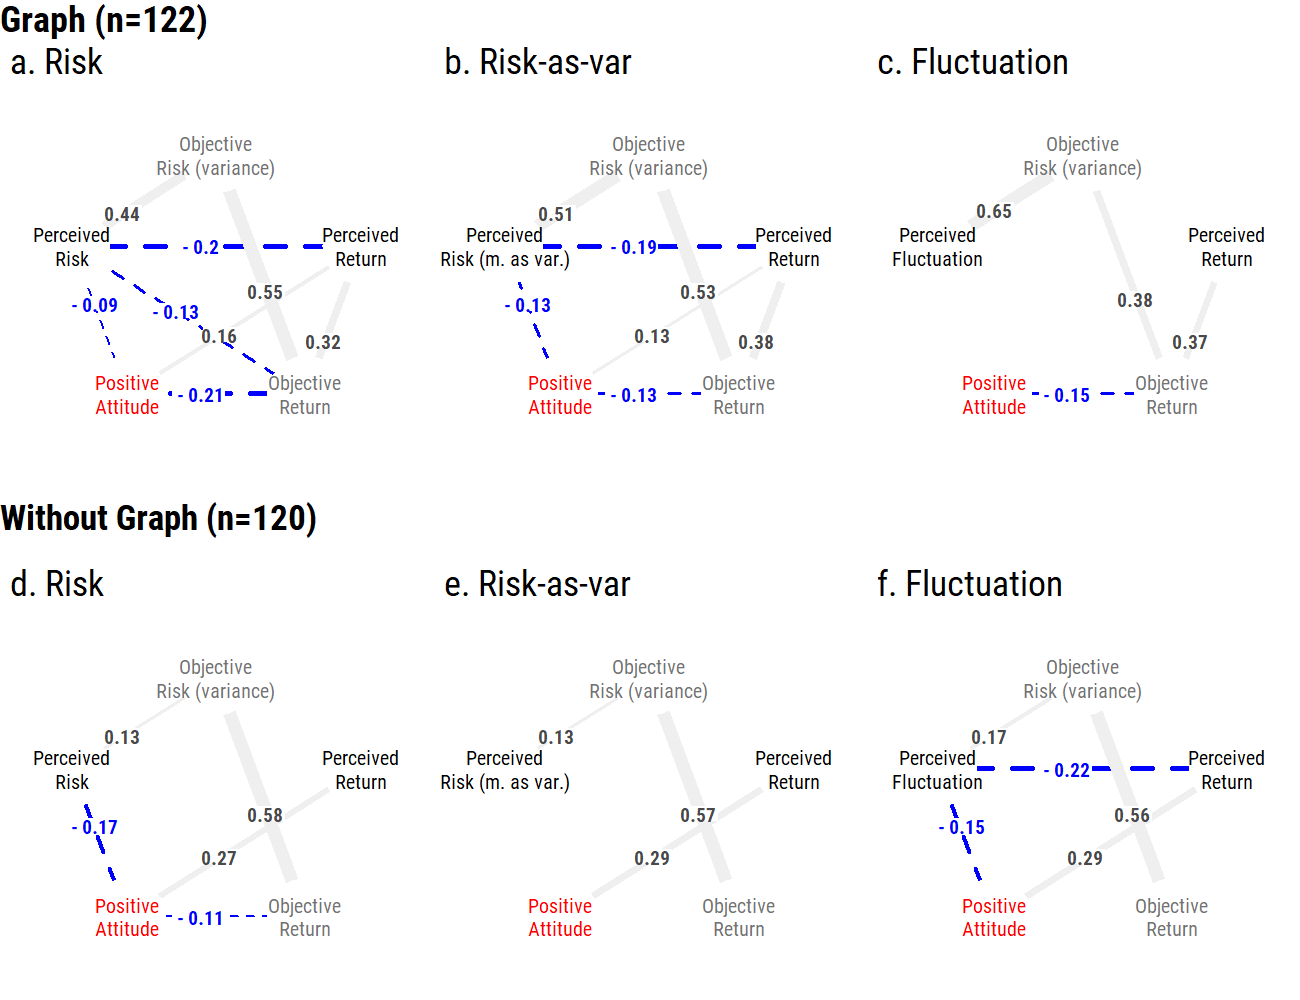
\includegraphics{fig8}
%     \caption{\textit{Study 2: The role of attitudes in the risk-return relationship.} Coefficients are partial correlations, only significant paths are shown, significance level: $0.05/6 = 0.0083$.}.
%     \label{fig:study2_pcor_attitudes}
% \end{figure}

% The results of Study~2 extend the findings of Study~1, that the risk-return paradox is influenced by the strong semantic connotation of the term term "risk" with loss, and further showed that this effect could not overcome by qualifying the term "risk" as meaning variance. The further highlight that without the availability of objective information about the characteristics of financial investment options, the risk and return beliefs are less accurate and biased independently the term chosen to measure variance of the funds.\footnote{The partial correlation networks used a by-participant random effect. In our data, participants repeatedly evaluated indices, and indices were repeatedly evaluated. To account for this fact, we also ran a hierarchical linear regression, with by-index and by-participant random effects (specification see Supplement \ref{tab:study2_lm_return_modelcomparison}), predicting the return perceptions as a function of variance perceptions interacting with the question wording and the graph presentation, while controlling for the objective variance and the objective return on the perceived return. By adding random effects by participant \textit{and} by index we maximized the random effects structure \citep[as recommended,][]{Barr2013}, and this also was the best-fitting model (AICs see Supplement \ref{tab:study2_lm_return_modelcomparison}). The results from this model confirm the partial correlation network analysis.}
%
% \begin{figure}[!htbp] 
%  \centering
%  \fitfigure[]{fig5.png} 
%   \caption{\textit{Study 2: Risk-return paradox.} Shown are the partial correlations among perceived risk (fluctuation) and return, controlling for the correlations between the other variables. \textit{Panel a-c} $=$  participants presented with return graphs; \textit{panel d-e} $=$ participants without return graphs; \textit{line width}$=$association strength; \textit{dashed lines} $=$ negative associations; \textit{missing lines} $=$  non-significant associations at $\alpha=.05/6 = .0083$ to correct for six comparisons. Shown are within-subject paths, i.e. how each subjects' deviations from the means predict each other for the same stock \citep[contemporeanous effects, ][]{Epskamp2018}).}
%   \label{fig:study2_partial_correlation_networks}
% \end{figure}

% To test if perceptions of investment risk and fluctuation are subject to the affect heuristic, we analyzed if attitudes mediates risk-return perceptions, conditional on showing return graphs. The affect heuristic  postulates that, given little information about the true risks, positive attitudes go along with higher perceived returns and lower perceived risks \citep{Finucane2000}. This means, attitudes are a source for the risk-return paradox.



% \begin{table}[tbp]
% \begin{center}
% \begin{threeparttable}
% \caption{Study 2: Goodness of fit of partial correlation networks.}
% \begin{tabular}{lllll}
% \toprule
%  & \multicolumn{2}{c}{Base
% Network Model} & \multicolumn{2}{c}{Base + Attitudes
% Network Model} \\
% \cmidrule(r){2-3} \cmidrule(r){4-5}
%  & AIC & BIC & AIC & BIC\\
% \midrule
% \multicolumn{5}{c}{Graph + Risk}\\
% Objective Risk (variance) & 2,060.80 & 2,102.50 & 2,062.85 & 2,113.81\\
% Perceived Return & 2,164.45 & 2,201.52 & 2,166.90 & 2,213.24\\
% Objective Return & 2,069.82 & 2,111.52 & 2,044.41 & 2,095.37\\
% Positive Attitude & 2,150.57 & 2,187.63 & 2,149.71 & 2,196.04\\
% Perceived Risk & NA & NA & 2,002.94 & 2,049.27\\
% \multicolumn{5}{c}{Risk (m. as var.)}\\
% Objective Risk (variance) & 2,158.77 & 2,200.91 & 2,161.28 & 2,212.78\\
% Perceived Return & 2,221.07 & 2,258.52 & 2,223.18 & 2,270.00\\
% Objective Return & 2,169.91 & 2,212.04 & 2,146.33 & 2,197.83\\
% Positive Attitude & 2,254.97 & 2,292.42 & 2,258.52 & 2,305.35\\
% Perceived Risk (m. as var.) & NA & NA & 2,167.24 & 2,214.06\\
% \multicolumn{5}{c}{Fluctuation}\\
% Objective Risk (variance) & 2,060.58 & 2,102.28 & 2,064.55 & 2,115.52\\
% Perceived Return & 2,142.09 & 2,179.15 & 2,144.72 & 2,191.06\\
% Objective Return & 2,074.01 & 2,115.71 & 2,050.59 & 2,101.55\\
% Positive Attitude & 2,134.32 & 2,171.39 & 2,137.99 & 2,184.32\\
% Perceived Fluctuation & NA & NA & 2,007.21 & 2,053.55\\
% \multicolumn{5}{c}{Without Graph + Risk}\\
% Objective Risk (variance) & 2,101.92 & 2,143.85 & 2,104.08 & 2,155.32\\
% Perceived Return & 2,218.19 & 2,255.45 & 2,220.41 & 2,266.99\\
% Objective Return & 2,090.01 & 2,131.93 & 2,074.28 & 2,125.52\\
% Positive Attitude & 2,201.89 & 2,239.15 & 2,200.58 & 2,247.16\\
% Perceived Risk & NA & NA & 2,052.05 & 2,098.63\\
% \multicolumn{5}{c}{Risk (m. as var.)}\\
% Objective Risk (variance) & 2,004.95 & 2,046.42 & 2,008.70 & 2,059.39\\
% Perceived Return & 2,107.03 & 2,143.89 & 2,109.02 & 2,155.10\\
% Objective Return & 1,995.02 & 2,036.49 & 1,964.68 & 2,015.37\\
% Positive Attitude & 2,104.49 & 2,141.35 & 2,099.70 & 2,145.78\\
% Perceived Risk (m. as var.) & NA & NA & 1,964.70 & 2,010.78\\
% \multicolumn{5}{c}{Fluctuation}\\
% Objective Risk (variance) & 2,048.10 & 2,089.80 & 2,052.06 & 2,103.03\\
% Perceived Return & 2,125.24 & 2,162.31 & 2,120.66 & 2,167.00\\
% Objective Return & 2,058.48 & 2,100.18 & 2,050.07 & 2,101.03\\
% Positive Attitude & 2,069.81 & 2,106.87 & 2,069.27 & 2,115.61\\
% Perceived Fluctuation & NA & NA & 2,054.48 & 2,100.82\\
% \bottomrule
% \end{tabular}
% \end{threeparttable}
% \end{center}
% \end{table}

% Figure~\ref{fig:study2_pcor_attitudes} shows the results of the partial correlation analysis of the perceived and objective variables including the attitude score. The results partially support the affect heuristic. We found the predicted positive attitude-return association in the no-graph condition for risk ($\rho=0.27, p<.001$), risk-as-variance ($\rho=.29, p<.001$), and fluctuation ($\rho=.29, p<.001$) and in the graph condition for risk ($\rho=0.16,p<.001$), risk-as-variance ($\rho=.13,p<.01$), but not for fluctuation ($\rho=.06, p=0.21$). However, the affect heuristic's prediction of a negative association between positive attitudes and risk/variance perception was supported in the risk condition (with graph: $\rho=-.09,p=0.016$, without graph: $\rho=-0.17, p<.001$), and in the risk-as-variance condition (with graph: $\rho=-0.13, p<.001$, without graph: $\rhos=-.11, p=0.03$), and in the fluctuation condition only without graph ($\rho=-.15,p<.001$). Note, this evidence is correlative without implications for causality.



Figure~\ref{fig:study2_mediation_paths} and Table~\ref{tab:study2_mediation} show the results of the mediation analysis regarding the influence of attitudes on the perceived risk-return relationship. The affect heuristic posits that stronger positive  attitudes produce a stronger risk-return paradox.
%, we used mediation analysis \citeauthor{Imai2010} (\citeyear{Imai2010})\footnote{
    % This method uses simulations to estimate mediation effects, which overcomes limitations of the traditional product-of-coefficients and difference-in-coefficients methods. See \citeauthor{Imai2010} (\citeyear{Imai2010}) for details. The method has the advantage of being able to control for clustering in the data by using by-participant random effects.  The model was specified as in footnote 12, but omitting the main effects, because we were interested in the mediation of the condition-perception interaction.
%and estimated using the mediation package version 4.4.7 \citep{tingeley2014}. The results 
We found a mediation only in the risk and risk-as-fluctuation condition, but for fluctuation attitudes suppressed an otherwise positive fluctuation-return association (with graphs). Regarding risk, more positive attitudes partially mediated the perceived risk-return relationships: "risk" had an unmediated effect of $b=-0.24, p=.009$ on return perceptions, which was weakened to $b=-0.20, p=.022$ through the mediator attitudes (with graphs). Perceived "risk (measured as variance)" had a negative but insignificant association with perceived returns originally ($b=-0.11$), but the effect size diminished significantly with the mediation ($b=−0.09$), with graphs, in line with the affect heuristic. Importantly, perceived "fluctuation" had a positive not substantial unmediated effect on return perception ($b=0.17$), which was not mediated but boosted by adding the indirect effect through affect ($b=0.19, p=.028$), with graphs. Thus, when measuring fluctuation, stronger positive attitudes suppressed a positive perceived fluctuation-return association. Therefore there is an interaction between attitudes and fluctuation perception, rather than a mediation of the fluctuation-return relationship through affect. This is only partially in line with the affect heuristic: when asking for "risk" and "risk (measured as variance)" we found support for the mediator affect as predicted by the affect heuristic, but when measuring variance perceptions by fluctuation, we found an interaction with attitudes.

\begin{figure}[H]
    \centering
    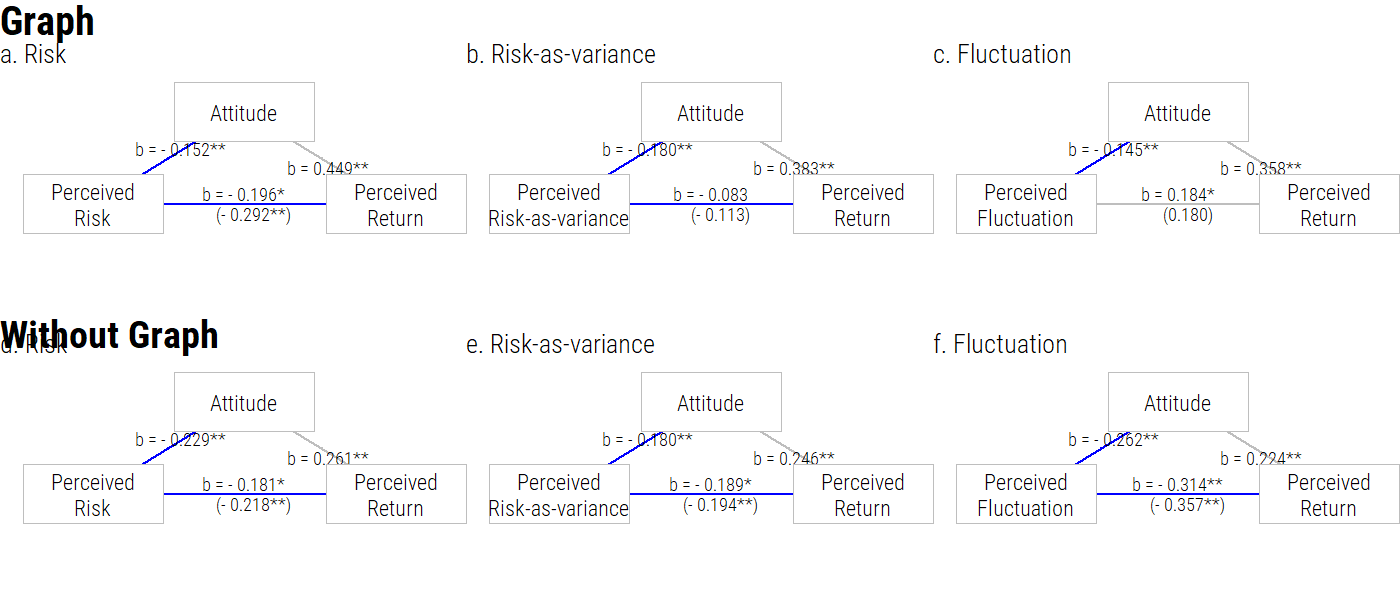
\includegraphics{fig7}
    \caption{\textit{Study 2: Attitude Mediation Effects by condition.} \textit{blue lines}$=$negative paths. More details, see text and mediation effects in Table~\ref{tab:study2_mediation}}.
    \label{fig:study2_mediation_paths}
\end{figure}



% and "risk (measured as variance)" the mediation exaggerates a direct negative effect, but regarding perceived "fluctuation" the mediation suppresses a direct positive effect. In other words, higher perceived risks decrease perceived returns---the risk-return paradox---and this effect becomes stronger through attitudes. However, higher perceived fluctuation increases perceived returns---in line with the objective risk premium---but attitudes have the opposite effect. Taken together, in the fluctuation condition, the mediation leads to a weak overall effect. This holds for the graph condition. In the condition without graphs (Table~\ref{tab:study2_mediation}), the mediation effect is negative across all wording conditions, and all direct effects---influence of perception on return perception independent of the mediation---are negative.



% \begin{figure}[H]
%     \centering
%     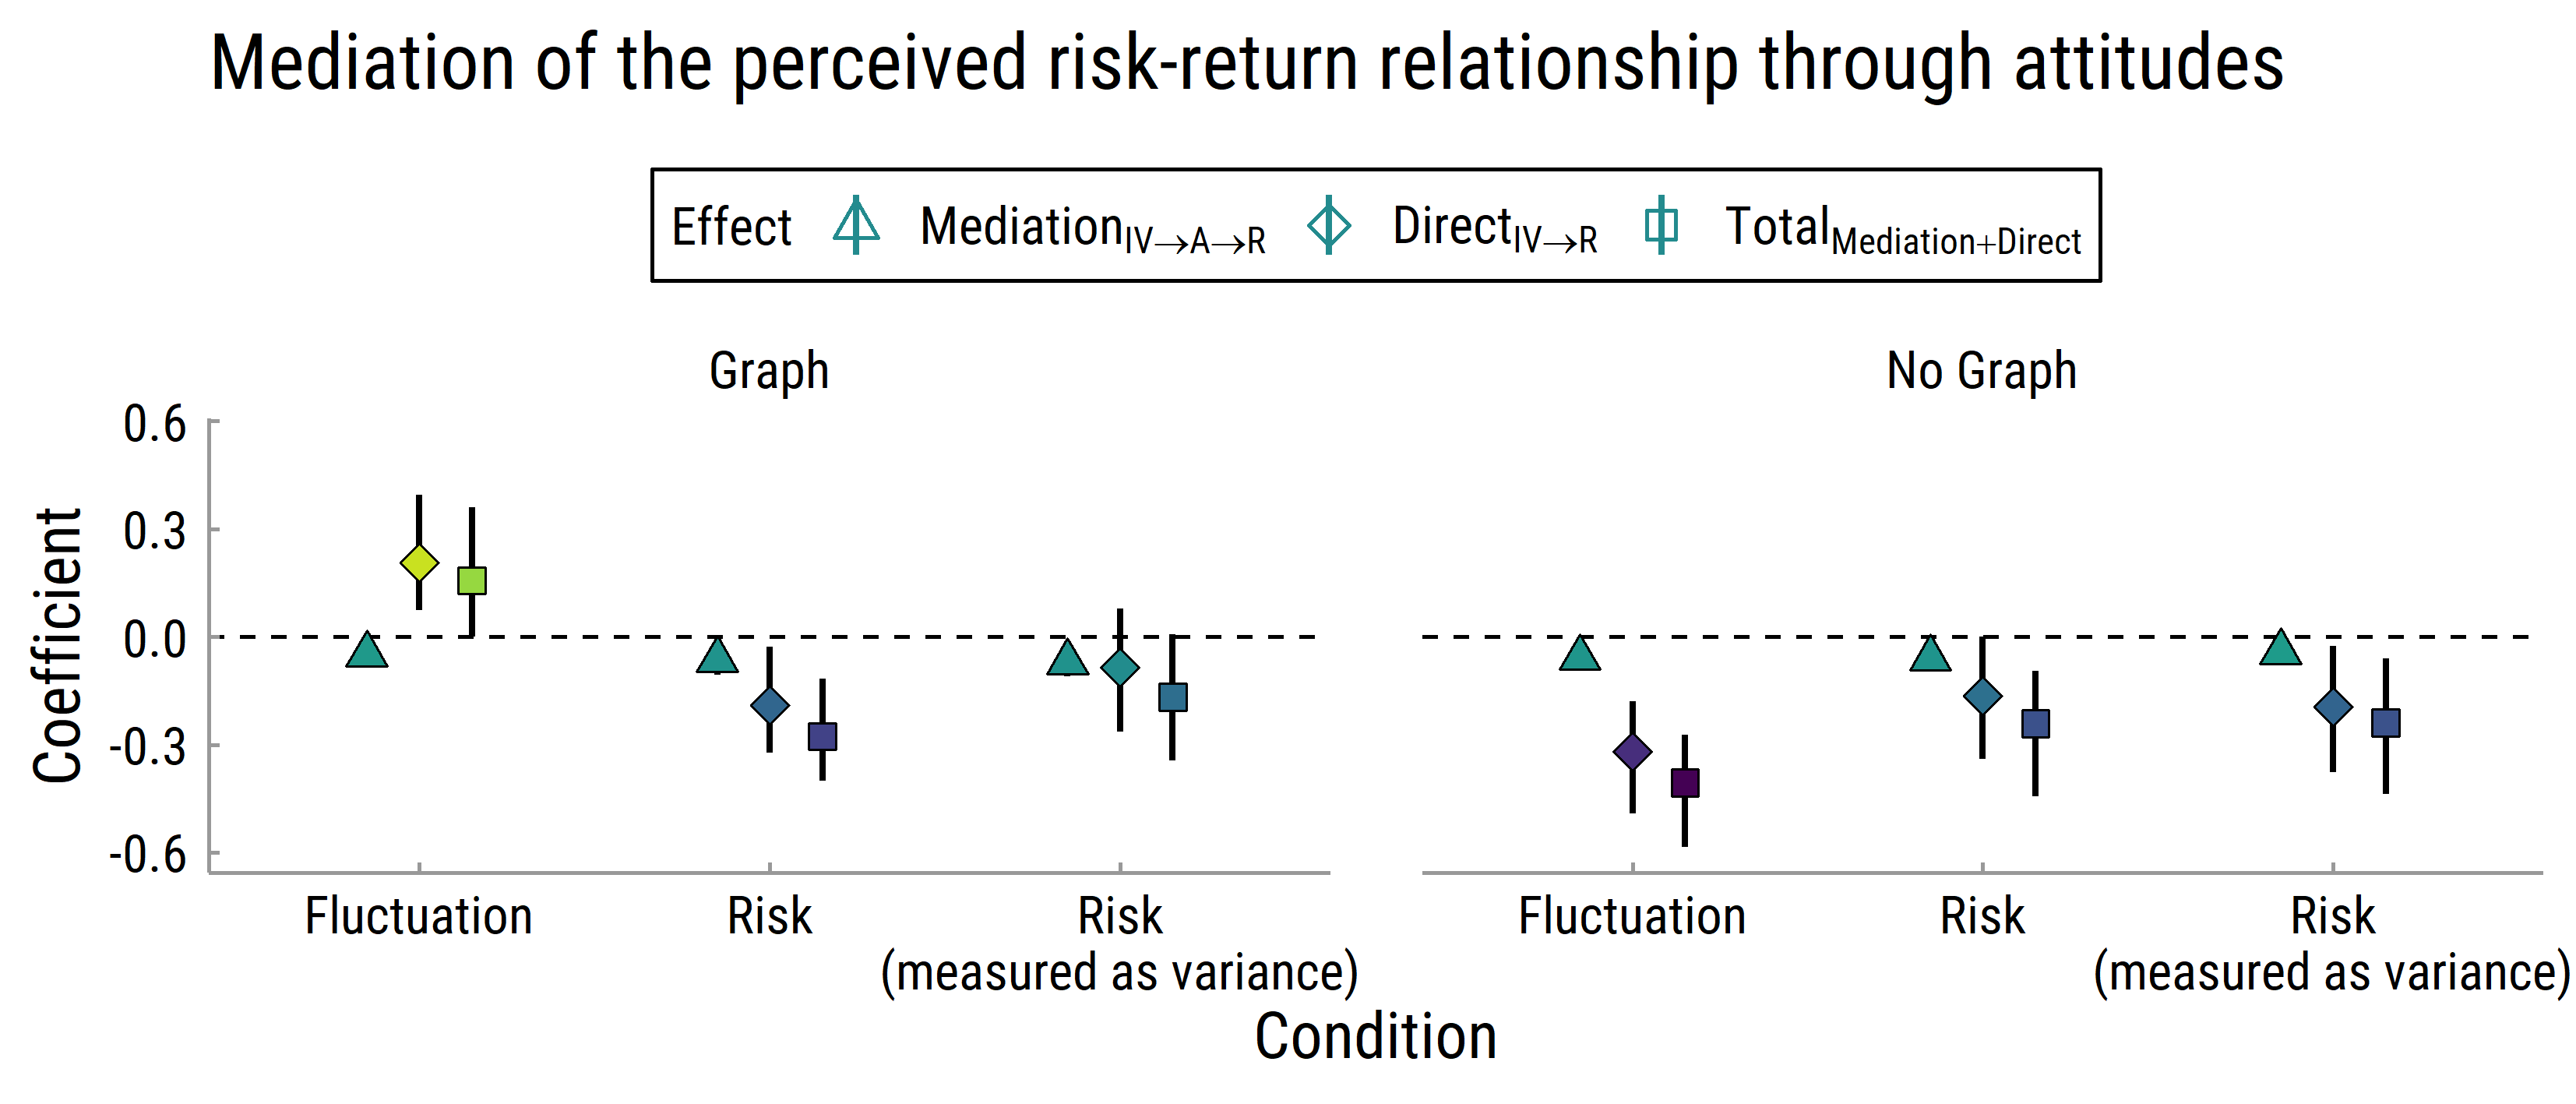
\includegraphics{fig6}
%     \caption{\textit{Study 2: Illustration of Attitude Mediation Effects by condition.} Attitude as mediator between independent variables (risk/fluctuation perception) and return perception. \textit{Mediation}$=$effect of independent variable on return perception through affect; \textit{Direct}$=$effect of independent variable on return perception not through affect; \textit{IV}$=$independent variable; \textit{A}$=$Affect, \textit{R}$=$Return perception. Error bars are 95\% CIs.}
%     \label{fig:study2_mediation}
% \end{figure}

\begin{table}[H]
\begin{threeparttable}
    
    \caption{\label{tab:study2_mediation}Mediation analysis, dependent variable: perceived risk; mediator: attitude score}
    \centering
    \fontsize{9}{10}\selectfont
    \begin{tabular}{@{}l@{\hspace{2mm}}r@{\hspace{2mm}}c@{\hspace{2mm}}r@{\hspace{4mm}}r@{\hspace{2mm}}c@{\hspace{2mm}}r@{\hspace{4mm}}r@{\hspace{2mm}}c@{\hspace{1mm}}r}
    \toprule
    \multicolumn{1}{c}{ } & \multicolumn{3}{c}{Mediaton Effect} & \multicolumn{3}{c}{Direct Effect} & \multicolumn{3}{c}{Total Effect} \\
    \multicolumn{1}{c}{ } & \multicolumn{3}{c}{IV $\rightarrow $ A $\rightarrow$ R} & \multicolumn{3}{c}{IV $\rightarrow$ R} & \multicolumn{3}{c}{} \\
    \cmidrule(l{3pt}r{3pt}){2-4} \cmidrule(l{3pt}r{3pt}){5-7} \cmidrule(l{3pt}r{3pt}){8-10}
      IV & \textit{b} & 95\% CI & \textit{p} & \textit{b} & 95\% CI & \textit{p} & \textit{b} & 95\% CI & $p$\\
    \midrule
    \addlinespace[0.3em]
    & \multicolumn{9}{c}{Graph}\\
    \cmidrule{2-10}
    Risk & $-$0.069 & [$-$0.11, $-$0.03] & $<$.001 & $-$0.200 & [$-$0.37, $-$0.03] & .022 & $-$0.295 & [$-$0.48, $-$0.12] & .004\\
    Risk (m. as var.) & $-$0.068 & [$-$0.10, $-$0.03] & $<$.001 & $-$0.088 & [$-$0.26, 0.08] & .326 & $-$0.167 & [$-$0.34, 0.00] & .062\\
    Fluctuation & $-$0.052 & [$-$0.09, $-$0.02] & $<$.001 & 0.187 & [0.01, 0.35] & .028 & 0.133 & [$-$0.04, 0.29] & .154\\
    \midrule
    & \multicolumn{9}{c}{No Graph}\\
    \cmidrule{2-10}
    Risk & $-$0.059 & [$-$0.09, $-$0.03] & $<$.001 & $-$0.176 & [$-$0.34, $-$0.01] & .042 & $-$0.256 & [$-$0.43, $-$0.08] & .002\\
    Risk (m. as var.) & $-$0.044 & [$-$0.07, $-$0.02] & $<$.001 & $-$0.182 & [$-$0.37, $-$0.01] & .032 & $-$0.230 & [$-$0.42, $-$0.06] & .008\\
    Fluctuation & $-$0.058 & [$-$0.09, $-$0.04] & $<$.001 & $-$0.314 & [$-$0.50, $-$0.13] & $<$.001 & $-$0.401 & [$-$0.59, $-$0.21] & $<$.001\\
    \addlinespace[0.3em]
    \bottomrule
    \end{tabular}
    \begin{tablenotes}\small
        \textit{Note.} \textit{IV}: Independent variables. \textit{Mediation Effect}: Indirect effect of the IV on return perception through the mediator attitudes, IV $\rightarrow$ A $\rightarrow$ R. \textit{Direct Effect}: Effect of the IV on return perception not transmitted through the mediator attitudes, IV $\rightarrow$ R. \textit{b}: unstandardized effects. Results are based on 1000 simulation runs per condition (6000 runs).
    \end{tablenotes}
\end{threeparttable}
\end{table}


%regression modeling of perceived return from wording, graph, and risk perception with index as random effect were fit using the afex package version 0.22 in R\footnote{Model specification: dependent variable perceived return (z-standardized at individual level), independent variables, fixed effects: graph, question wording, risk perception, and the interactions of them, random effects: random slope by index.}; adding attitudes improved the model fit compared to a model without attitudes (AIC$_{simple}=12910$, AIC$_{attitudes}=12840$, LL$_{simple}=-6440.9$, LL$_{attitudes}=-6394.2$, $\chi^2=93.48, p$<$.001$). attitudes values were z-standardized to ease interpretation of lower-order effects, which now can be interpreted as the effect at the mean attitudes. Importantly, even if attitudes is added as predictor, the fluctuation remains positively correlated with 




%We compared people's response frequencies to the attitudesive rating scales with a Chi square test (XXXX Hoffentlich nicht. Falls nicht. We cannot reject the null hypothesis, suggesting that generally, people's attitudesive attitude towards the countries does not differ between conditions. ).

%Figure XXX displays people's attitudesive ratings split by company and scale (rows). Table \ref{table:cor.attitudes} shows how responses to the different scales were correlated. The correlation coefficiens are XXX and range from -.66 to .58. In contrast to \cite{Kempf2014a}, active -- which supposedly has a positive connotation --  was negatively associated with all other \textit{positive} notions. To account for this fact, we recoded the active/passive scale such that passive was positively connoted and active negatively connoted. \footnote{Hier Literatur hin, die zeigt, dass aktiv nicht immer eindeutig gut ist. Sarah hat dazu mal Literatur gesucht, müssen sie mal fragen.}.

% \subsection{The influence of familiarity on the perception of risk and return} Familiarity has been identified as a booster for the negative perceived risk-return relationship \citep{Ganzach2000}. Study~2 elicited self-reported familiarity with all funds (How well do you know the fund x? 1=\textit{not at all} through 3=\textit{medium} to 7$=$\textit{very well}). The median familiarity was 2 (\textit{M}$=$2.29, \textit{SD}$=$1.5, range 1--7). The index fund most-familiar to participant was ES50 from Europe (\textit{M}$=$3.75), the least familiar fund was KLSE from Malaysia (\textit{M}$=$1.72).

\subsection{Discussion of Study 2}
In summary, the results from Study~2 show that when participants have information about the underlying return paths, the risk-return paradox prevails even if qulifying the term "risk" as "risk (measured as variance)". What de-biased the risk-return relationship, however, was asking about perceived fluctuation. Attitudes mediated the strength of the risk-return paradox only when asking about risk: more positive attitudes exaggerated a negative perceived risk-return relationship but suppressed a positive fluctuation-return relationship. If, however, participants could not base their judgments on graphical information about the stock returns, they believed that higher returns are negatively related to risk, fluctuation, and risk (measured as variance). It is therefore important to provide fundamental information in addition to labels when communicating investment risks. 

\section{General Discussion}
Risk is a rich and ambiguous term in everyday language. This research investigate the role of the semantics of the term risk in the assessment and communication of risk (variance) and return in the financial domain. We showed that the meaning of risk as related to losses substantially influences people's perception of the variances and returns of financial investment options. In particular, the common perception that higher risks imply lower returns (the risk-return paradox), which is often interpreted as cognitive bias, was driven by an interaction of attitudes and the semantic of risks. Importantly, substituting the ambiguous term risk by a more clear term in the measurement of risk perceptions eliminated the risk-return paradox, given that participants were not guessing the variance and returns. This means that people did not fundamentally mis-perceive the relationship between the variance and return of the investment options, but correctly perceived the risk premium. The risk-return paradox is thus a by-product of the loss-semantic of risk. The belief in the meaning of risk as loss---not variance---caused a paradoxical negative perceived risk-return correlation. Our second contribution is that the results indicate that substituting questions about risk by questions about fluctuation lead to more accurate and less biased perceptions of variances from financial information. The finding that the most accurate elicitation of beliefs about the real risks (variances) of financial investments is produced by asking about fluctuation is important for practitioners and risk perception researchers. The third contribution concerns the influence of affect and information. Affect influences the risk-return paradox, as predicted by the affect heuristic, if measuring risk. Regarding information, in order to de-bias the risk-return paradox, it is necessary to provide information about past performance of financial products rather than mere labels of financial investment options.

The findings described above show how the belief that risk relates to losses even if risk is explicitly defined to mean variance. This finding is in line with the literature on the usage of risk in everyday language \citep{Boholm2016} and with recent literature linking psychological risk aversion to loss aversion \citep{Duxbury2004}. The semantic mix-up of risk with loss causes the psychological risk-return paradox, namely a negative perceived risk-return correlation when in fact the true risk-return correlation is positive. In two experiments we have shown that the allegedly erroneous belief in a negative risk-return relationship vanishes when people are asked to report fluctuation of assets rather than risk and when people are not guessing the properties of the assets but judge them from fundamental information. We interpret this finding as that the strong connotation of risk with loss is partially responsible for the risk-return paradox. 

The present results, that the loss-semantics of risk biases risk judgments is important, because common assessment of risk perception uses the term risk \citep[e.g.,][]{Socio-EconomicPanelSOEP2012}, often in a single item \citep[e.g.,][]{Keller2006}. Our findings regarding that risk judgments increase in accuracy if measured by "fluctuation" instead of "risk" suggests that---if variance perception is the target---the term "risk" should be substituted by terms without loss semantics, for example by "fluctuation".

The finding that risk judgments are influenced by loss perceptions can provide an explanation why risk judgments are less stable over time than benefit judgments \citep{Connor2016}. They also establish loss aversion as one important psychological factor of human risk (variance) perception in addition to the factor attitudes \citep{Finucane2000, Slovic2007}. Our data show support for the affect heuristic, but at the same time they show that removing the connotation of risk with loss not merely reduced the risk-return paradox---which is expected when controlling for attitudes---but completely reverted the negative perceived risk-return correlation. This large effect suggest that many psychological features that are commonly attributed to risk psychology may actually be the psychology of losses.

There are some limitations of the current work. One of our key results concerns information: in the absence of any information about the performance of the stocks, participants perceptions of risk were inaccurate for all terms used to assess risk (variance) perceptions. This means that using unambiguous terminology alone will not guarantee good risk comprehension in the absence of further information. Moreover, our study design focused on financial risk perception. It is not clear if the strong influence of loss semantics on risk perception that we found here, holds across domains, where risk perceptions have been shown to differ systematically \citep{Weber2002, Wilke2014}. Also, our study investigated the affect heuristic, but not other psychological factors like representativeness \citep[e.g.,][]{Shefrin1995}, or familiarity \citep[e.g.,][{Weber2005}, which have been shown to influence risk perceptions.

In sum, our findings question the adequacy of questions about "risk" in the assessment of the perceived variance of options with probabilistic outcomes. As previously established, risk to laypeople means variability, loss, and uncertainty. This is in line with analyses of the usage of "risk" in everyday language. We believe that common cognitive biases in "risk" perception may be caused by that while in academia, risk has a clear definition as variance, in non-academic language risk is an ambiguous term.  We have shown that if information is available, one such risk perception paradox---the risk-return paradox---turns out as a by-product of people confusing the concept of risk with the concept of loss.



\bibliography{references.bib,refJanine.bib}

\appendix
\title{Supplementary Material}
% \section{Practical Relevance}
% \label{postfinance}

% \begin{figure}[!htbp] 
% \centering
% 
\includegraphics[width=.8\linewidth, keepaspectratio]{Postfinance_Risk_2018Jun19.png} 
% \caption{Information about the risks, that is variance, associated with an investment fund, taken from the consumer webpage of a major Swiss bank (accessed 19. June 2017). The bank explains that "The risk classification is based on the fluctuation range (volatility) of the fund. PostFinance takes the view that risks are very high from a level of 20\% or more. A fund may however be subject to considerably greater fluctuation. The maximum level shown is 20\%"}
% \label{fig:pfrisk}
% %POSTFINANCE:
% % https://www.postfinance.ch/pfch-web/feed-direct/postfinance/vfund/CH0006869207_en.pdf?method=pdf&isin=CH0006869207&lang=en
% % The risk classification is based on the fluctuation range (volatility) of the fund. PostFinance takes the view that risks are very high from a level of 20% or more. A fund may however be subject to considerably greater fluctuation. The maximum level shown is 20%.

% % https://www.postfinance.ch/en/private/products/investing-trading/fund-range.html/feed/fragment/postfinance/fragment2016/funds/fundDetail.jsp?valor=686920&market=393&currency=CHF 
% % retrieved 5.9.2017; 16:58
% \end{figure}

\section{Study 1 Supplementary Material}
\subsection{Materials Used in Study 1}
\label{sup:study1_material}
\textit{Stimuli.} The materials used in Study~1 were the annual returns on investment of stocks of 20 companies. Data about the start and closing values between 2002 and 2015 were obtained. The stocks were the 20 most-traded Swiss stocks at the time of the study (2016), which were CS Group N,
ABB N,
Swiss Re N,
UBS Group N,
Adecco Group N,
LafargeHolcim N,
Nestle N,
Novartis N,
Swiss Life Hldg N,
Richemont N,
Actelion N,
Syngenta N,
Roche Hldg DR,
Givaudan N,
Geberit N,
The Swatch Grp,
Swisscom Reg,
SGS Reg,
Zurich Insur Grp N,
(Julius Baer Grp N),
and SMI.
The stock of Julius Baer was excluded because the available return time series started only in 2009. Note that the names of the stocks were not shown to participants. 

\textit{Question wording for variance.} The original question wording (German) of the variance-related questions read as follows: (a, risk) Wie hoch schätzen Sie das Risiko der gezeigten Aktie ein?  (b, variability) Wie hoch schätzen Sie die Variabilität (Varianz) der gezeigten Aktie ein? (c, fluctuation) Wie hoch schätzen Sie die durchschnittliche Schwankung der Rendite der gezeigten Aktie ein? (d, predictability) Wie hoch schätzen Sie die Vorhersagbarkeit der Rendite der gezeigte Aktie ein (gemessen ab 2003)?

\textit{Question wording for gain/loss.} The gain- and loss-related questions read as follows: (a) Wie hoch schätzen Sie den erwarteten durchschnittlichen Verlust (in \%-Punkten) für diese Aktien ein? (b) Wie hoch schätzen Sie den durchschnittlichen Verlust (in \%-Punkten) für die Jahre, in denen die gezeigte Aktie Verluste erzielt hat, ein? (c) Wie hoch schätzen Sie die Wahrscheinlichkeit ein mit der gezeigten Aktie in einem zufällig ausgewähltem Jahr einen Verlust (negative Rendite) zu erzielen? (d) Wie hoch schätzen Sie die durchschnittliche Rendite der gezeigten Aktie ein? (extrem hoher verlust, extrem hoher gewiance Correlations

\subsection{Supplementary Results, Study 1}
\label{study1_supplementary_results}
\textit{Risk--variance correlation}
\label{study1_risk-variance-correlation}
Correlations between the objective variance and the perceptions of fluctuation, risk, predictability, and variability of the stocks used in Study~1 are shown in Table A1. Simple correlations (pooled across stimuli and participants) between objective outcome variance and perceived fluctuation are shown in Table \ref{{sup:tab:study1_rvc}}.
\begin{table}[]
    \centering
    \begin{threeparttable}
    \caption{Study 1: Simple correlations between the objective risk (variance) and the perceptions of stocks}
    \label{sup:tab:study1_rvc}
    \begin{tabular}{lrcrr}\toprule
         & $r$ &  95\% CI & $t$ & $p$ \\
          \midrule
        Perceived fluctuation & $.69$ & $[.67$, $.72]$ & $t(1822) = 41.02$ & $< .001$ \\
        Perceived variation & $.64$ & $[.61$, $.66]$ &  $t(1822) = 35.23$ & $< .001$\\
        Perceived predictability & $-.52$ &  $[-.56$, $-.49]$ & $t(1822) = -26.29$ &  $< .001$\\
        Perceived risk & $.49$ & $[.45$, $.52]$ & $t(1822) = 24.02$ & $< .001$\\
        \bottomrule
    \end{tabular}
    \begin{tablenotes}
    \textit{Note.} CI = Confidence interval. Perceived values are \textit{z} standardized at the individual level.
    \end{tablenotes}
    \end{threeparttable}
\end{table}

\begin{table}[H]
\begin{center}
\begin{threeparttable}
\caption{Study 1: Simple correlations between perceived return and perceived variance
  \label{sup:tab:study1_rrc}}
\begin{tabular}{llrrll}
\toprule
 & \textit{r} & CI 1 & CI 2 & \textit{t} & \textit{p}\\
\midrule
Fluctuation & .11 & .07 & .16 & 4.75 & .00\\
Risk & -.14 & -.18 & -.09 & -5.90 & .00\\
Variability & .10 & .06 & .15 & 4.36 & .00\\
Predictability & -.03 & -.08 & .01 & -1.38 & .17\\
\bottomrule
\addlinespace
\end{tabular}
\begin{tablenotes}[para]
\normalsize{\textit{Note.} CI = Confidence interval. Pearson correlations $r$ from pooled data; subjective values are \textit{z} standardized at the individual level.}
\end{tablenotes}
\end{threeparttable}
\end{center}
\end{table}


For mixed-effects models, it is recommended to report the variance--covariance matrix \cite{Barr2013}. For the model of perceived risk as function of different perceptions of variance, the variance--covariance matrix is shown in Table~\ref{sup:tab:study_1_vcovmat}. 

\begin{table}[H]
\begin{center}
\begin{threeparttable}
\caption{Study 1: Variance--covariance matrix of the mixed-effects model with dependent variable perceived return}
\label{sup:tab:study_1_vcovmat}
\begin{tabular}{llllll}
\toprule
 & \multicolumn{1}{c}{(1)} & \multicolumn{1}{c}{(2)} & \multicolumn{1}{c}{(3)} & \multicolumn{1}{c}{(4)} & \multicolumn{1}{c}{(5)}\\
\midrule
(1) Constant & 0.006 &  &  &  & \\
(2) Perception & 0.000 & 0.000 &  &  & \\
(3) Perception:Risk & 0.000 & 0.000 & 0.001 &  & \\
(4) Perception:Fluctuation & 0.000 & 0.000 & 0.000 & 0.001 & \\
(5) Perception:Variability & 0.000 & 0.000 & 0.000 & 0.000 & 0.001\\
\bottomrule
\addlinespace
\end{tabular}
\begin{tablenotes}[para]
\normalsize{\textit{Note.}  The colons denote interaction terms. For model specification, see footnotes in the main text. Predictors were \textit{z} standardized at the individual level.}
\end{tablenotes}
\end{threeparttable}
\end{center}
\end{table}

\subsubsection{Study 1: Partial correlation details}
Table~\ref{tab:study1_pcc} shows the numerical details of the partial correlation analysis, that is, all coefficients and the $p$ values obtained from fitting the partial correlation networks (for implementation details, see main text). Shown are the coefficients for the perceived "risk," "fluctuation," "variability," and "predictability" and the objective risk (variance) and return of the stocks shown during Study~1.

\begin{table}[H]
\begin{center}
\begin{threeparttable}
\caption{\label{tab:study1_pcc}Study 1 results: Partial correlations and \textit{p} values from the correlation networks
\label{study1_pcc}}
\begin{tabular}{rccc}
\toprule
 & \multicolumn{1}{c}{Objective risk (variance)} & \multicolumn{1}{c}{Perceived return} & \multicolumn{1}{c}{Objective return}\\
\midrule
\cmidrule{2-4} \textbf{ Perceived risk } &  &  & \\
\ \ \ Objective risk (variance) & --- &  & \\
\ \ \ Perceived return & \textbf{.09}, $p<.001$ & --- & \\
\ \ \ Objective return & \textbf{.38}, $p<.001$ & \textbf{.30}, $p<.001$ & ---\\
\ \ \ Perceived risk & \textbf{-.08}, $ p= .00 $ & \textbf{-.15}, $p<.001$ & \textbf{-.07}, $ p= .00 $\\
\cmidrule{2-4} \textbf{ Perceived fluctuation } &  &  & \\
\ \ \ Objective risk (variance) & --- &  & \\
\ \ \ Perceived return & \textbf{.10}, $p<.001$ & --- & \\
\ \ \ Objective return & \textbf{.39}, $p<.001$ & \textbf{.32}, $p<.001$ & ---\\
\ \ \ Perceived fluctuation & -.04, $ p= .08 $ & -.05, $ p= .09 $ & \textbf{.21}, $p<.001$\\
\cmidrule{2-4} \textbf{ Perceived variability } &  &  & \\
\ \ \ Objective risk (variance) & --- &  & \\
\ \ \ Perceived return & \textbf{.11}, $p<.001$ & --- & \\
\ \ \ Objective return & \textbf{.39}, $p<.001$ & \textbf{.33}, $p<.001$ & ---\\
\ \ \ Perceived variability & -.03, $ p= .26 $ & -.07, $ p= .02 $ & \textbf{.22}, $p<.001$\\
\cmidrule{2-4} \textbf{ Perceived predictability } &  &  & \\
\ \ \ Objective risk (variance) & --- &  & \\
\ \ \ Perceived return & \textbf{.10}, $p<.001$ & --- & \\
\ \ \ Objective return & \textbf{.39}, $p<.001$ & \textbf{.32}, $p<.001$ & ---\\
\ \ \ Perceived predictability & \textbf{.09}, $p<.001$ & .04, $ p= .19 $ & -.06, $ p= .02 $\\
\bottomrule
\addlinespace
\end{tabular}
\begin{tablenotes}[para]
\normalsize{\textit{Note.} Boldface $=$ significant partial correlations at $\alpha= 0.0125 $.}
\end{tablenotes}
\end{threeparttable}
\end{center}
\end{table}

\newpage
\subsubsection{Robustness Check I: Graph literacy}
Figure~\ref{fig:study1_pcor_by_glit} shows the significant partial correlations after splitting the data at the median graph literacy.
\begin{figure}[H] 
 \centering
 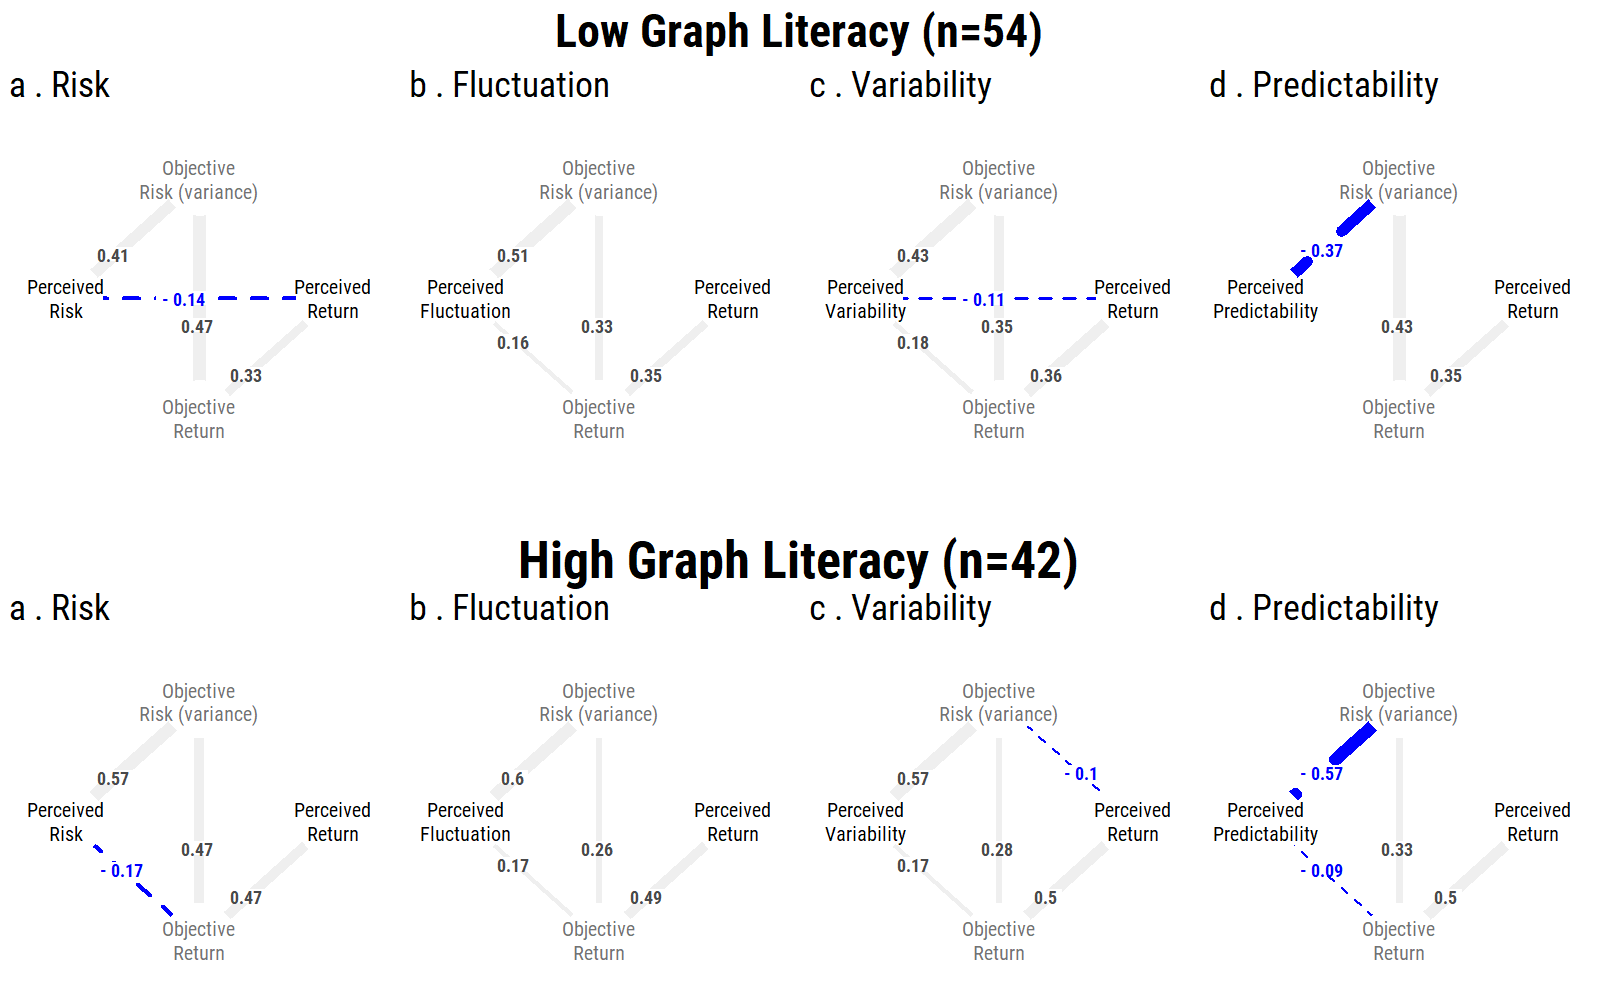
\includegraphics[width=.8\linewidth, keepaspectratio]{sfig1.png} 
 \caption{Partial correlation network. The methodology is similar to as described in the main text for Study 1, split by graph literacy. Only significant edges are shown, $\alpha=.01$.}
 \label{fig:study1_pcor_by_glit}
\end{figure}

\subsubsection{Robustness Check II: Stock market experience}
Figure~\ref{fig:study1_pcor_by_exp} shows the significant partial correlations after splitting the data into participants relatively inexperienced with the stock market and those with experience.
\begin{figure}[H] 
 \centering
 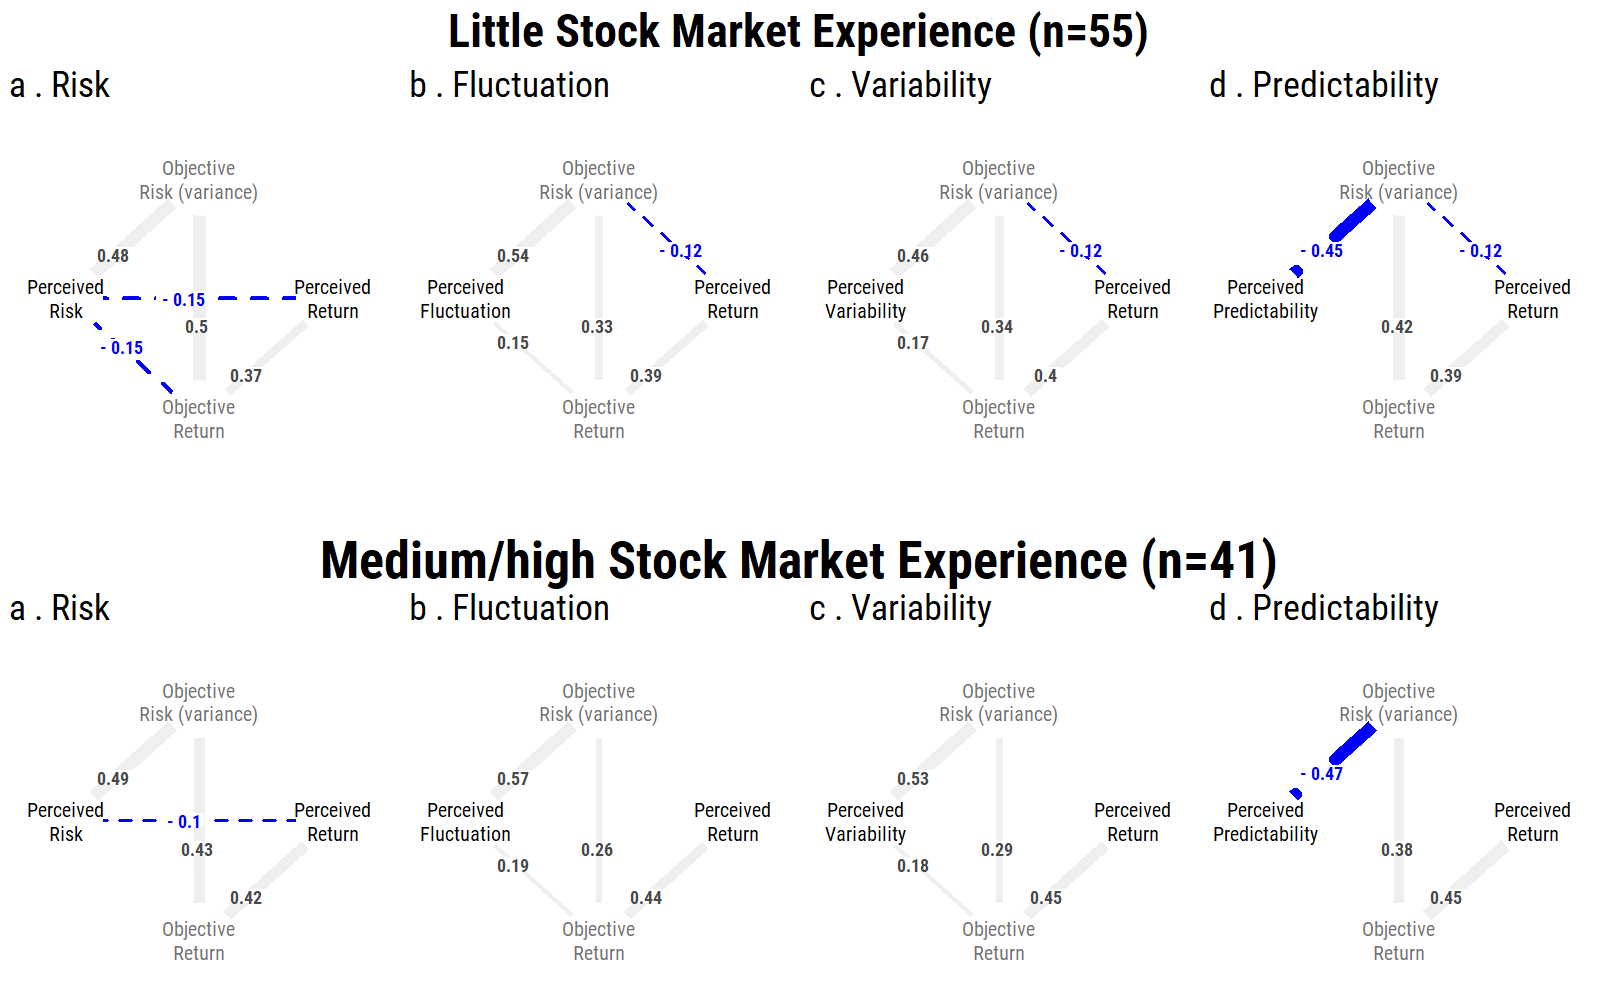
\includegraphics[width=.8\linewidth, keepaspectratio]{sfig2.png} 
 \caption{Partial correlation network. The methodology is similar to as described in the main text for Study 1, split by experience with the stock market. Only significant edges are shown, $\alpha=.01$.}
 \label{fig:study1_pcor_by_exp}
\end{figure}




%%%%%%%%%%%%%%%%%%%%%%%%%%%%%%%%%%%%%%%%%%%%%%%%%%%%%%%%%%%%%%%%%%%%%%%%%%%%%%%%%%%%%%%%%%





\section{Study 2 Supplementary Material}
\subsection{Materials Used in Study 2}
\label{tab:study2_material}
For Study 2, data from 1 January 2009 through 1 August 2017 from price indices of 23 stock markets corresponding to the world's most traded currencies (as of 2017) were obtained. Only price indices were used. Price indices calculate the value of the index based on the value of the stocks, excluding dividends. Table~\ref{tab:study2_material} lists the indices used in our study. Note: The HSI index (China-Hong Kong, Hang Seng Index) was excluded in favor of the Shanghai Stock Exchange Composite Index (SSE Composite), to avoid China being the only country to appear twice in the stimulus material. Also, the German DAX index was excluded in favor of the European EUROSTOXX index, which is also traded in euros. This table shows only the abbreviated version of the stimuli.
% latex table generated in R 3.5.0 by xtable 1.8-3 package
% Fri May 10 15:54:55 2019
\begin{table}[ht]
\centering\small
\caption{Stocks used in Study~2} 
\label{tab:study2_material}
\begin{tabularx}{.6\textwidth}{lcc}
  \toprule
Country & Index fund & ISIN \\ 
  \midrule
Europe & ES50 (EuroStoxx50) & EU0009658145 \\ 
  USA & DJIA & US2605661048 \\ 
  Japan & Nikkei225 & JP9010C00002 \\ 
  United Kingdom & FTSE100 & GB0001383545 \\ 
  Switzerland & SMI20 & CH0009980894 \\ 
  Australia & ASX & XC0009693018 \\ 
  Canada & TSX & XC0009695252 \\ 
  China-Shanghai & SSEC & CNM000000019 \\ 
  Sweden & OMXS30 & SE0000337842 \\ 
  Singapore & FSSTI & XC0009653640 \\ 
  India & BSE & XC0009698199 \\ 
  Russia & RTSI & RU000A0JPEB3 \\ 
  South Africa & JSE (JALSH) & --- \\ 
  Turkey & ISE100 & TRAIMKB00010 \\ 
  Poland & WIG20 & PL9999999987 \\ 
  Argentina & MERV & ARMERV160025 \\ 
  Indonesia & IDX & --- \\ 
  Malaysia & KLSE & --- \\ 
  Norway & OBX & NO0007035376 \\ 
  Mexico & MXX & --- \\ 
   \bottomrule
\end{tabularx}
\begin{tablenotes}
    \textit{Note.} ISIN $=$ International Securities Identification Number
\end{tablenotes}
\end{table}



\subsection{Supplementary Analyses, Study 2}
\label{sup:study2_results}
\subsubsection{Correlation coefficients}
\label{study2_subj_obj_cor}
Table~\ref{tab:study2_subj_obj_cor} shows the correlations between the objective variances of the returns of the index funds and the three perceptions of the variances: risk, fluctuation, and risk (measured as variance), pooled across participants and stimuli. This does not take the clustered nature of the data into account; see below for results controlling for the clustering. The simple correlation is highest for perceptions of fluctuation.
%
\begin{table}[H]
\begin{center}
\begin{threeparttable}
\caption{Study 2: Simple correlations between perceived risk and objective risk (variance)}
\label{tab:study2_subj_obj_cor}
\begin{tabular}{lrcrr}
\toprule
  & $r$ & 95\% CI & $t$ & $p$\\
 \midrule
& \multicolumn{4}{c}{Graph}\\
\cmidrule{2-5}
 Perceived risk (measured as variance) & $-.10$ & $[-.16$, $-.03]$ & $t(838) = -2.85$ & $.004$\\
 Perceived risk & $-.19$& $[-.26$, $-.12]$ & $t(798) = -5.54$& $<.001$\\
 Perceived fluctuation & $.19$ & $[.12$, $.25]$ & $t(798) = 5.41$& $<.001$\\
\midrule
 & \multicolumn{4}{c}{No graph}\\
 \cmidrule{2-5}
 Perceived risk (measured as variance) & $.19$ & $[-.26$, $-.12]$ & $t(778) = -5.47$& $ <.001$\\
 Perceived fluctuation & $-.39$ & $[-.44$, $-.33]$ & $t(798) = -11.81$& $ <.001$\\
 Perceived risk & $-.22$ & $[-.28$, $-.15]$ & $t(818) = -6.33$&  $ <.001$\\
\bottomrule
\addlinespace
\end{tabular}
\begin{tablenotes}[para]
\normalsize{\textit{Note.} CI = Confidence interval; Pearson correlations $r$ from pooled data; subjective values \textit{z} standardized at the individual level.}
\end{tablenotes}
\end{threeparttable}
\end{center}
\end{table}


\subsubsection{Study 2: Objective variance and subjective judgments, pairwise post hoc comparisons}
Table~\ref{tab:study2_hlm_trends_pairwise} shows the post hoc pairwise contrasts between the obtained regression coefficients, regressing objective variance on ratings of risk, fluctuation, and risk (variance), using Tukey \textit{p}-value adjustments. When graphs are shown, fluctuation perceptions are correlated strongest with the objective outcome variances of the index funds, compared with risk or risk (variance) perceptions, albeit the effect is small.
% latex table generated in R 3.6.0 by xtable 1.8-4 package
% Mon Jun 17 13:19:48 2019
\begin{table}[H]
\centering
\caption{Pairwise comparisons between trend coefficients with dependent variable: objective risk (variance of the index funds)} 
\label{tab:study2_hlm_trends_pairwise}
\begin{threeparttable}

    
    \begin{tabular}{lrrrrl}
      \toprule
    Contrast & $\Delta$ Slope & \textit{SE} & \textit{df} & $z$ Ratio & $p$ \\ 
      \midrule
      & \multicolumn{5}{c}{Graph}\\
      \cmidrule{2-6}
    Risk (variance)---fluctuation & -0.029 & 0.006 & Inf & -4.934 & $<$.0001 \\ 
      Risk (variance)---risk & 0.010 & 0.006 & Inf & 1.621 & .2366 \\ 
      Fluctuation---risk & 0.039 & 0.006 & Inf & 6.477 & $<$.0001 \\ 
       \midrule
       & \multicolumn{5}{c}{No graph}\\
       \cmidrule{2-6}
    Risk (variance)---fluctuation & -0.014 & 0.006 & Inf & -2.312 & .0542 \\ 
      Risk (variance)---risk & -0.006 & 0.006 & Inf & -0.991 & .5828 \\ 
      Fluctuation---risk & 0.008 & 0.006 & Inf & 1.344 & .3708 \\ 
       \bottomrule
    \end{tabular}
    \begin{tablenotes}
    \textit{Note.} Slope based on unstandardized effects; \textit{p}-value adjustment: Tukey for comparing three estimates. Inf $=$ Infinite.
    \end{tablenotes}
    \end{threeparttable}
\end{table}


% Table created by stargazer v.5.2.2 by Marek Hlavac, Harvard University. E-mail: hlavac at fas.harvard.edu
% Date and time: Mi., Mai 08, 2019 - 16:56:38
\begin{table}[!htbp] \centering \small
 \caption{Study 2: Linear mixed model results with dependent variable: objective variance of shown stocks} 
 \label{table:supplement_tab1} 
\begin{tabular}{@{\extracolsep{5pt}}lccc} 
\\[-1.8ex]\hline 
\hline \\[-1.8ex] 
 & \multicolumn{3}{c}{Unstandardized \textit{b} coefficients [range of dependent variable: 0.14--0.60]} \\ 
\cline{2-4} 
\\[-1.8ex] & (1) & (2) & (3)\\ 
\hline \\[-1.8ex] 
 Graph & $-$0.00 & $-$0.00 & \\ 
 & ($-$.01, .01) & ($-$.01, .01) & \\ 
 & $t$ = $-$0.00 & $t$ = $-$0.00 & \\ 
 & & & \\ \midrule
 Risk $\times$ No graph & .04 & & .05 \\ 
 & (.03, .05) & & (.04, .06) \\ 
 & $t$ = 9.59$^{***}$ & & $t$ = 16.89$^{***}$ \\ 
 & & & \\ 
 Risk (variance) $\times$ No graph & .03 & & .05 \\ 
 & (.03, .04) & & (.05, .06) \\ 
 & $t$ = 7.93$^{***}$ & & $t$ = 17.79$^{***}$ \\ 
 & & & \\ 
 Fluctuation $\times$ No graph & .05 & & .07 \\ 
 & (.04, .06) & & (.07, .08) \\ 
 & $t$ = 11.41$^{***}$ & & $t$ = 24.74$^{***}$ \\ 
 & & & \\ 
 Risk (all) $\times$ No graph & & .04 & \\ 
 & & (.04, .04) & \\ 
 & & $t$ = 16.62$^{***}$ & \\ 
 & & & \\ \midrule
 Risk$^{a}$ $\times$  Graph & .02 & .08 & \\ 
 & (.01, .03) & (.07, .08) & \\ 
 & $t$ = 3.69$^{***}$ & $t$ = 32.21$^{***}$ & \\ 
 & & & \\ 
 Risk (variance) $\times$ Graph & .02 & & \\ 
 & ($-$.001, .03) & & \\ 
 & $t$ = 1.89 & & \\ 
 & & & \\ 
 Fluctuation $\times$ Graph & .03 & & \\ 
 & (.01, .05) & & \\ 
 & $t$ = 3.74$^{***}$ & & \\ 
 & & & \\ \midrule
 Constant & .28 & .28 & .28 \\ 
 & (.28, .29) & (.28, .29) & (.28, .29) \\ 
 & $t$ = 121.40$^{***}$ & $t$ = 120.73$^{***}$ & $t$ = 170.06$^{***}$ \\ 
 & & & \\ 
\hline \\[-1.8ex] 
AIC weight$^{b}$ & 1.00 & 0.00 & 0.00 \\ 
AIC & -7,242 & -7,197 & -7,118 \\ 
BIC & -7,177 & -7,158 & -7,079 \\ 
LogLik & 3,631 & 3,604 & 3,565 \\ 
Random slope & no & no & no \\ 
Random intercept & participant & participant & participant \\ 
\hline 
\hline \\[-1.8ex] 
\multicolumn{4}{l}{\textit{Note.} $^{*}$ \textit{p} $<$ .05; $^{**}$\textit{p} $<$ .01; $^{***}$\textit{p} $<$ .001. Predictors are \textit{z} transformed.} \\
  \multicolumn{4}{l}{$^{a}$For Model 2, the predictor "risk" refers to all question wordings.} \\ 
 \multicolumn{4}{l}{$^{b}$Relative evidence strength, range 0 to 1 {\citep{Wagenmakers2004}}} \\
\end{tabular} 
\end{table} 



\subsubsection{Study 2: The risk--return paradox}
Table~\ref{tab:study2_rr} shows the simple correlation coefficients between the perceived return and the perceived risk/risk-as-variance/fluctuation. Note, correlations are pooled (ignoring the repeated-measure data structure) and simple (ignoring the intercorrelations between the risk and return variables in the data).
% latex table generated in R 3.6.0 by xtable 1.8-4 package
% Mon Jun 17 16:02:01 2019
\begin{table}[h!t]
\centering
\caption{Correlation between perceived risk and objective risk (variance)}
\label{tab:study2_rr}
\begin{tabular}{llrr}
 Graph & Question wording & $r$ [95\% CI] & Statistic \\ 
  \midrule
Graph & Risk (variance) & $-.10$, \  $[-.16$, $-.03]$ & $t(838) = -2.85$, $p = .004$ \\ 
   & Risk & $-.19$, \  $[-.26$, $-.12]$ & $t(798) = -5.54$, $p < .001$ \\ 
   & Fluctuation & $.19$, \  $[.12$, $.25]$ & $t(798) = 5.41$, $p < .001$ \\ 
   \midrule
No Graph & Risk (variance) & $-.19$, \  $[-.26$, $-.12]$ & $t(778) = -5.47$, $p < .001$ \\ 
   & Fluctuation & $-.39$, \  $[-.44$, $-.33]$ & $t(798) = -11.81$, $p < .001$ \\ 
   & Risk & $-.22$, \  $[-.28$, $-.15]$ & $t(818) = -6.33$, $p < .001$ \\ 
   \bottomrule
\multicolumn{4}{l}{{\textit{Note.} CI = Confidence interval. Pearson correlations $r$ from pooled data; subjective values \textit{z} standardized at the individual level.}}
\end{tabular}
\end{table}







\newpage
\subsection{Partial correlation coefficients}
Table~\ref{tab:study2_pcc} shows the numerical details of the partial correlation analysis, that is, the coefficients and the $p$ values from fitting the partial correlation networks (for implementation details, see main text). Shown are the coefficients for the perceived "risk," "fluctuation," and  "risk (measured as variance)" and returns of the index funds that were rated during Study~2.


\begin{sidewaystable}                                                                   

\begin{TableNotes}[para]                                                                                                                                        
\normalsize{\textit{Note.}  $^{*} = \textit{p} < .05; ^{**} = \textit{p} < .01; ^{***} = \textit{p} < .001$.}                                                                       
\end{TableNotes}                                                                                                                                                
                                                                                                                                                                
\small{                                                                                                                                                         
                                                                                                                                                                
\begin{longtable}{lllllllll}\noalign{\getlongtablewidth\global\LTcapwidth=\longtablewidth}                                                                      
\caption{Study 2 results: Partial correlations and \textit{p} values from the correlation networks                                                                      
\label{tab:study2_pcc}}\\                                                                                                                                           
\toprule                                                                                                                                                        
 \multicolumn{4}{c}{Graph} & \multicolumn{4}{c}{No graph}  &\\                                                                                        
\cmidrule(r){1-4} \cmidrule(r){5-8}                                                                                                                             
 & \multicolumn{1}{c}{1} & \multicolumn{1}{c}{2} & \multicolumn{1}{c}{3} & \multicolumn{1}{c}{4} & \multicolumn{1}{c}{1} & \multicolumn{1}{c}{2} & \multicolumn{1}{c}{3} & \multicolumn{1}{c}{4}\\                                                                                                                              
\midrule                                                                                                                                                        
\endfirsthead                                                                                                                                                   
\caption*{\normalfont{Table \ref{tab:} continued}}\\                                                                                                            
\toprule                                                                                                                                                        
 \multicolumn{4}{c}{With graph} & \multicolumn{4}{c}{Without graph}  &\\                                                                                        
\cmidrule(r){1-4} \cmidrule(r){5-8}                                                                                                                             
 & \multicolumn{1}{c}{1} & \multicolumn{1}{c}{2} & \multicolumn{1}{c}{3} & \multicolumn{1}{c}{4} & \multicolumn{1}{c}{1} & \multicolumn{1}{c}{2} & \multicolumn{1}{c}{3} & \multicolumn{1}{c}{4}\\                                                                                                                              
\midrule                                                                                                                                                        
\endhead                                                                                                                                                        
Risk &  &  &  &  &  &  &  & \\                                                                                                                                  
\ \ \ 1 Perceived risk &  &  &  &  &  &  &  & \\                                                                                                                
\ \ \ 2 Perceived return & $-.20^{**}$ &  &  &  & $-.14$ &  &  & \\                                                                                           
\ \ \ 3 Objective risk (variance) & $\hphantom{-}.44^{***}$ & $-.01$ &  &  & $\hphantom{-}.13^{***}$ & $\hphantom{-}.02$ &  & \\                            
\ \ \ 4 Objective return & $-.13^{**}$ & $\hphantom{-}.32^{***}$ & $\hphantom{-}.55^{***}$ &  & $\hphantom{-}.02$ & $-.02$ & $\hphantom{-}.58^{***}$ & \\ 
\ \ \ 5 Positive attitude & $-.09^{*}$ & $\hphantom{-}.16^{***}$ & $\hphantom{-}.03$ & $-.21^{***}$ & $-.17^{***}$ & $\hphantom{-}.27^{***}$ & $-.01$ & $-.11^{**}$\\                                                                                                                                                   
Risk-as-variance &  &  &  &  &  &  &  & \\                                                                                                                      
\ \ \ 1 Perceived risk-as-variance &  &  &  &  &  &  &  & \\                                                                                                    
\ \ \ 2 Perceived return & $-.19^{**}$ &  &  &  & $-.11$ &  &  & \\                                                                                           
\ \ \ 3 Objective risk (variance) & $\hphantom{-}.51^{***}$ & $\hphantom{-}.05$ &  &  & $\hphantom{-}.13^{**}$ & $\hphantom{-}.00$ &  & \\                  
\ \ \ 4 Objective return & $-.10^{*}$ & $\hphantom{-}.38^{***}$ & $\hphantom{-}.53^{***}$ &  & $\hphantom{-}.08^{*}$ & $-.05$ & $\hphantom{-}.57^{***}$ & 
\\                                                                                                                                                              
\ \ \ 5 Positive attitude & $-.13^{**}$ & $\hphantom{-}.13^{**}$ & $-.03$ & $-.13^{***}$ & $-.11^{*}$ & $\hphantom{-}.29^{***}$ & $-.01$ & $-.08^{*}$\\ 
Fluctuation &  &  &  &  &  &  &  & \\                                                                                                                           
\ \ \ 1 Perceived fluctuation &  &  &  &  &  &  &  & \\                                                                                                         
\ \ \ 2 Perceived return & $\hphantom{-}.07$ &  &  &  & $-.22^{***}$ &  &  & \\                                                                               
\ \ \ 3 Objective risk (variance) & $\hphantom{-}.65^{***}$ & $-.10^{*}$ &  &  & $\hphantom{-}.17^{***}$ & $-.02$ &  & \\                                   
\ \ \ 4 Objective return & $\hphantom{-}.04$ & $\hphantom{-}.37^{***}$ & $\hphantom{-}.38^{***}$ &  & $\hphantom{-}.05$ & $-.08$ & $\hphantom{-}.56^{***}$ & \\                                                                                                                                                           
\ \ \ 5 Positive attitude & $-.09^{*}$ & $\hphantom{-}.06$ & $\hphantom{-}.05$ & $-.15^{***}$ & $-.15^{**}$ & $\hphantom{-}.29^{***}$ & $-.03$ & $-.09^{*}$\\                                                                                                                                                           
\bottomrule                                                                                                                                                     
\addlinespace                                                                                                                                                   
\insertTableNotes                                                                                                                                               
\end{longtable}                                                                                                                                                 
                                                                                                                                                                
}

\end{sidewaystable}






\subsubsection{Linear model comparison for perceived return}
Data-driven selection of the (hierarchical) linear model that we used in the main text was based on complexity-penalized goodness of fit (Akaike information criterion). Dependent variable was perceived return, and the fixed effects were Question $\times$ Perceived Variance, Graph $\times$ Perceived Variance, objective variance, and objective return. Predictors question and graph were effects coded. The random effects structure is varied: See the different rows in Table B7, where Row 1 contains a fixed-effects-only model and the last row the maximum random effects structure of interest. For all models, variance inflation factors ($VIF$) were at maximum 2 ($VIF > 5$ indicates problematic multicollinearity). Table \ref{sup:tab:study2_attitude_lm_trends} further displays the mixed-effects modeling results including the predictor attitudes.
% latex table generated in R 3.6.0 by xtable 1.8-4 package
% Fri Jun 21 08:49:47 2019
\begin{table}[H]
\centering
\caption{Study 2: Linear model comparison with dependent variable: perceived return} 
\label{tab:study2_lm_return_modelcomparison}
\begin{tabular}{p{4.3cm}cccccccr}
  \toprule
 & \textit{df} & AIC & BIC & LogLik & Deviance & $\chi^2$ & $\chi^2$\textit{df} & Pr(>$\chi^2$) \\ 
  \midrule
Fixed effects only & 10 & 14,791 & 14,855 & -7,385 & 14,771 &  &  &  \\ 
  Interc. by id & 11 & 14,504 & 14,575 & -7,241 & 14,482 & 289 & 1 & 0.000 \\ 
  Interc. by index & 11 & 14,612 & 14,683 & -7,295 & 14,590 & 0 & 0 & 1.000 \\ 
  Interc. \& slope by id & 13 & 13,517 & 13,601 & -6,745 & 13,491 & 1,099 & 2 & 0.000 \\ 
  Interc. \& slope by index & 13 & 14,611 & 14,695 & -7,293 & 14,585 & 0 & 0 & 1.000 \\ 
  Interc. \& slope by id + interc. \& slope by index & 16 & 13,308 & 13,412 & -6,638 & 13,276 & 1,309 & 3 & 0.000 \\ 
   \bottomrule
   \multicolumn{9}{l}{\small\textit{Note}. Variables were centered at the Likert scale midpoints. AIC = Akaike information criterion; BIC = Bayesian information criterion, id = participant identifyer, interc = intercept.}\end{tabular}
\end{table}


\begin{table}[H]
\begin{center}
\begin{threeparttable}
\caption{Study 2 results: Mixed-effects model with estimated slopes for the predictor attitude. Dependent variable: perceived return}
\label{sup:tab:study2_attitude_lm_trends}
\begin{tabular}{lccrrr}
\toprule
Question & Slope & \textit{SE} & \textit{df} & \textit{z} Ratio & \textit{p}\\
\midrule
& \multicolumn{5}{c}{No Graph}\\
\cmidrule{2-6}
Risk & 0.344 & 0.044 & \$\textbackslash{}infty\$ & 7.819 & .000\\
Risk (measured as variance) & 0.358 & 0.043 & \$\textbackslash{}infty\$ & 8.323 & .000\\
Fluctuation & 0.448 & 0.047 & \$\textbackslash{}infty\$ & 9.511 & .000\\
\midrule
& \multicolumn{5}{c}{Graph}\\
\cmidrule{2-6}
Risk & 0.145 & 0.041 & \$\textbackslash{}infty\$ & 3.501 & .000\\
Risk (measured as variance) & 0.085 & 0.041 & \$\textbackslash{}infty\$ & 2.087 & .037\\
Fluctuation & 0.077 & 0.038 & \$\textbackslash{}infty\$ & 2.058 & .040\\
\bottomrule
\end{tabular}
\begin{tablenotes} \small
    \textit{Note.} Model specification as in Footnote 12 of the main text, but adding to the fixed effects the attitude score as main effect and as interaction term.
\end{tablenotes}
\end{threeparttable}
\end{center}
\end{table}


\end{document}
